\documentclass{article}
\usepackage[english,american]{babel}
\usepackage{graphicx}
\usepackage{todonotes}
\usepackage{subfiles}
\usepackage{grffile}
\usepackage{booktabs}
\usepackage{hyperref}
\usepackage{fullpage}

\usepackage{csquotes}% Recommended
\usepackage{amssymb}
\usepackage[citestyle=numeric-comp,url=false,hyperref=auto,isbn=false]{biblatex}
\addbibresource{connectomics motif.bib}
\addbibresource{connectomics motif-relational models.bib}


\usepackage{amsmath}
\usepackage{subcaption}

\usepackage[firstpage]{draftwatermark}
\SetWatermarkScale{4}


\DeclareGraphicsRule{.ai}{pdf}{.ai}{}


\title{Spatial Relational Models for Neural Circuit Discovery}
\author{Eric Jonas \\ Konrad Kording}

\begin{document}
\maketitle

\listoftodos

\begin{abstract}
  The role of ``type''
  Clustering in molecular biology
\end{abstract}

\section{Introduction}

Things I believe

\begin{itemize}
\item The rise of complex data demands better computational tools to ``see'' into it
\item Clustering has worked for molecular biology and genetics
\item ``Type'' is a useful concept for understanding how neurobiological systems work
\item Many things people do with graphs are boring, not biologically relevant
\item Neuroanatomy needs to be a computational field
\end{itemize}

\section{Methods}
Stochastic blockmodels have been around forever, assume a latent ``type'' dictates
the probability of a latent class. We use recently-developed infinite
stochastic block models that 

\begin{figure}
  \centering 
  \begin{subfigure}[b]{0.4\textwidth}
    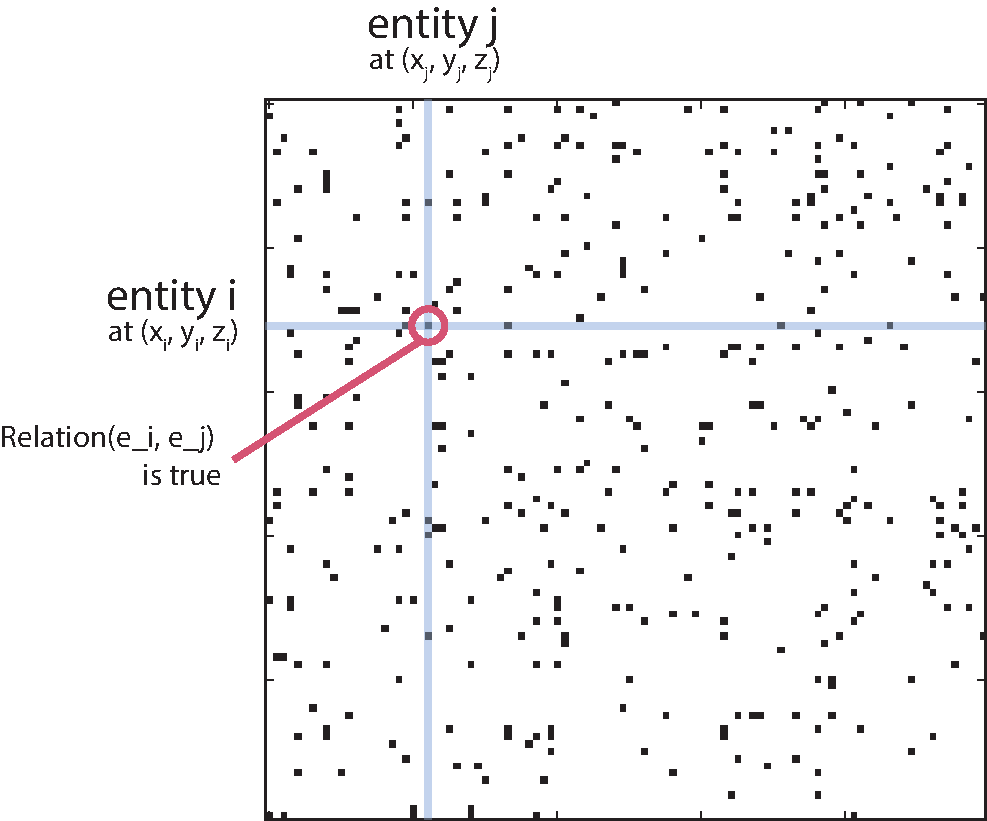
\includegraphics[width=\textwidth]{f1.raw.pdf}
    \caption{Raw data}
    \label{fig:gull}
  \end{subfigure}
  \begin{subfigure}[b]{0.55\textwidth}
    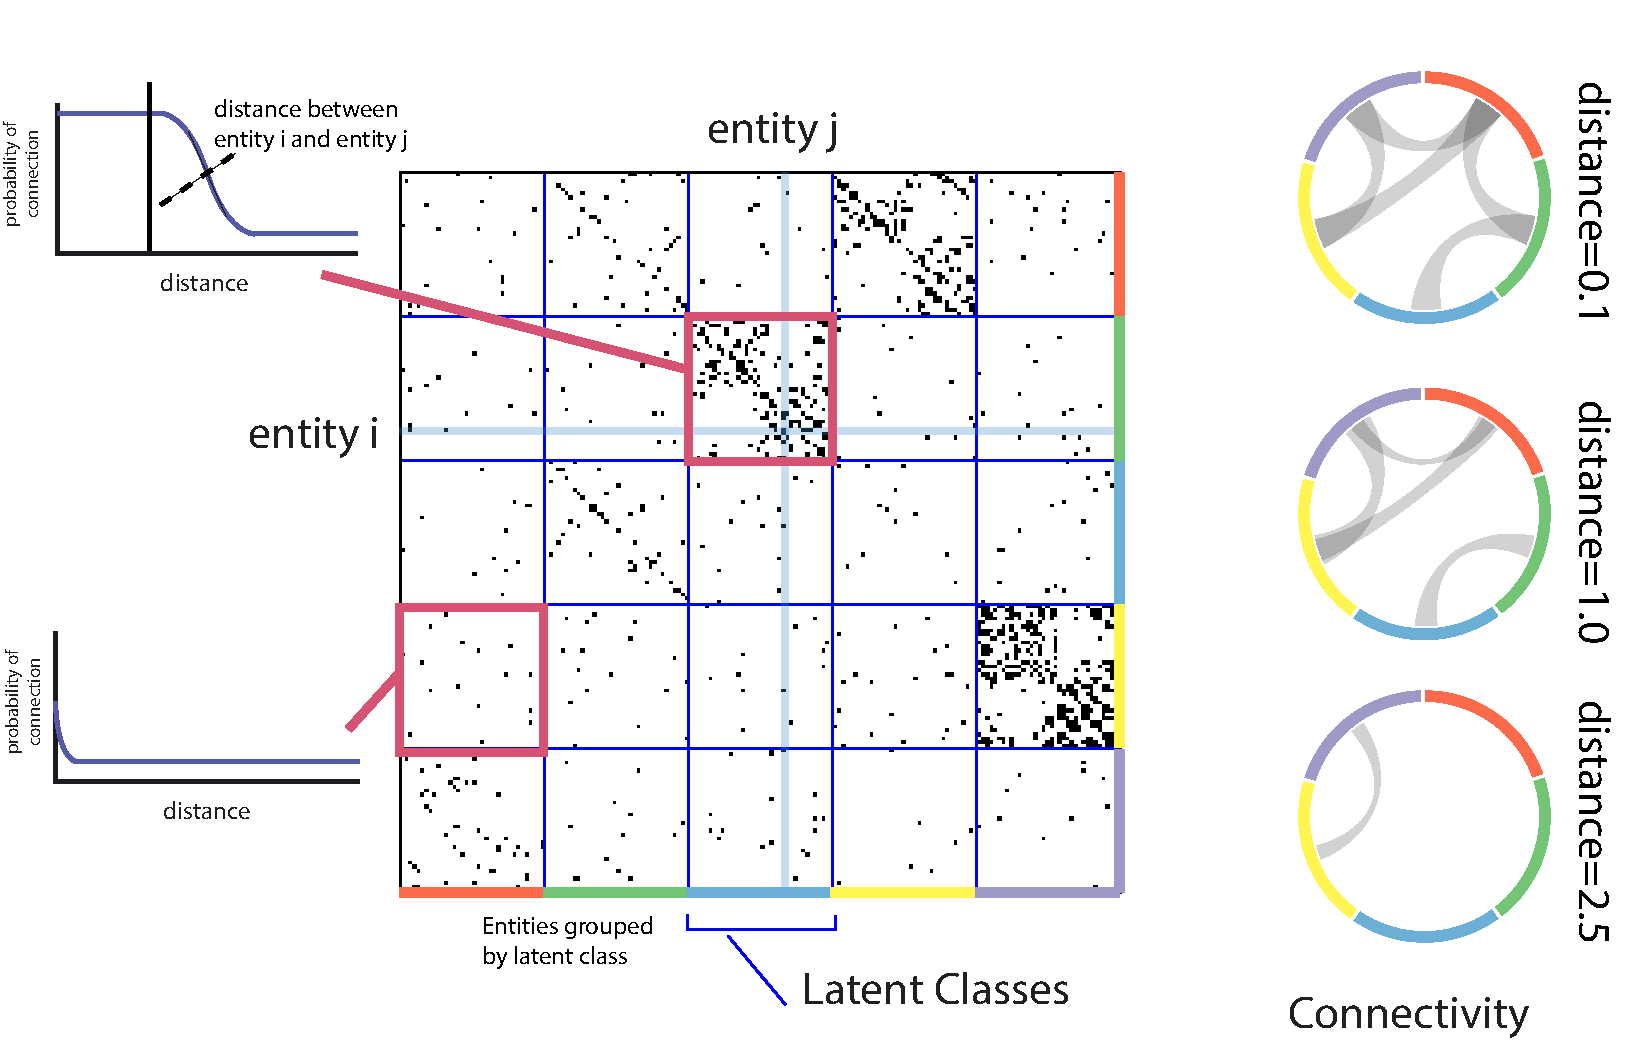
\includegraphics[width=\textwidth]{f1.sorted.pdf}
    \caption{Raw data}
    \label{fig:gull}
  \end{subfigure}
\end{figure}

\subsection{Infinite Spatial Relational Models}

We adopt the terminology from \autocite{Kemp2006a}. A domain $T_n$ is a
collection of entities $\{e^t_i | i \in 0 \dots N^t -1 \} $ that share
some common property. A relation is a collection of observation
defined on a collection of domains. For example, if one domain is
``students'' and another is ``courses'', the relation
``$\operatorname{has-taken}(e^s_i, e^c_j)$ is true if student $e^s_i$ has
taken course $e^c_j$. 

Our model assumes that the probabiltiy of a relation taking on a
particular observed value is only a function of some hidden ``type''
(or class, or cluster) of an entity. Each entity can belong to a
single latent class.

That is, if $e^1_i$ is an entity
in domain $T^1$ and in latent class $m$ and $e^2_j$ is an entity in
domain $T^2$ in latent class $n$, then 
\begin{equation}
\operatorname{Relation}(e^1_i, e^2_j) \sim F(\cdot | \eta_{mn})
\end{equation}

where $\eta_{mn}$ is an unobserved (latent) parameter.
\todo{Better framing of this}

Note that this framework is equivalent to the classic stochastic block
model, defined on a graph -- a relation $\operatorname{has-edge}(e_i,
e_j)$ is defined on the domain $T1$ of nodes. 

\begin{figure}
  \centering
  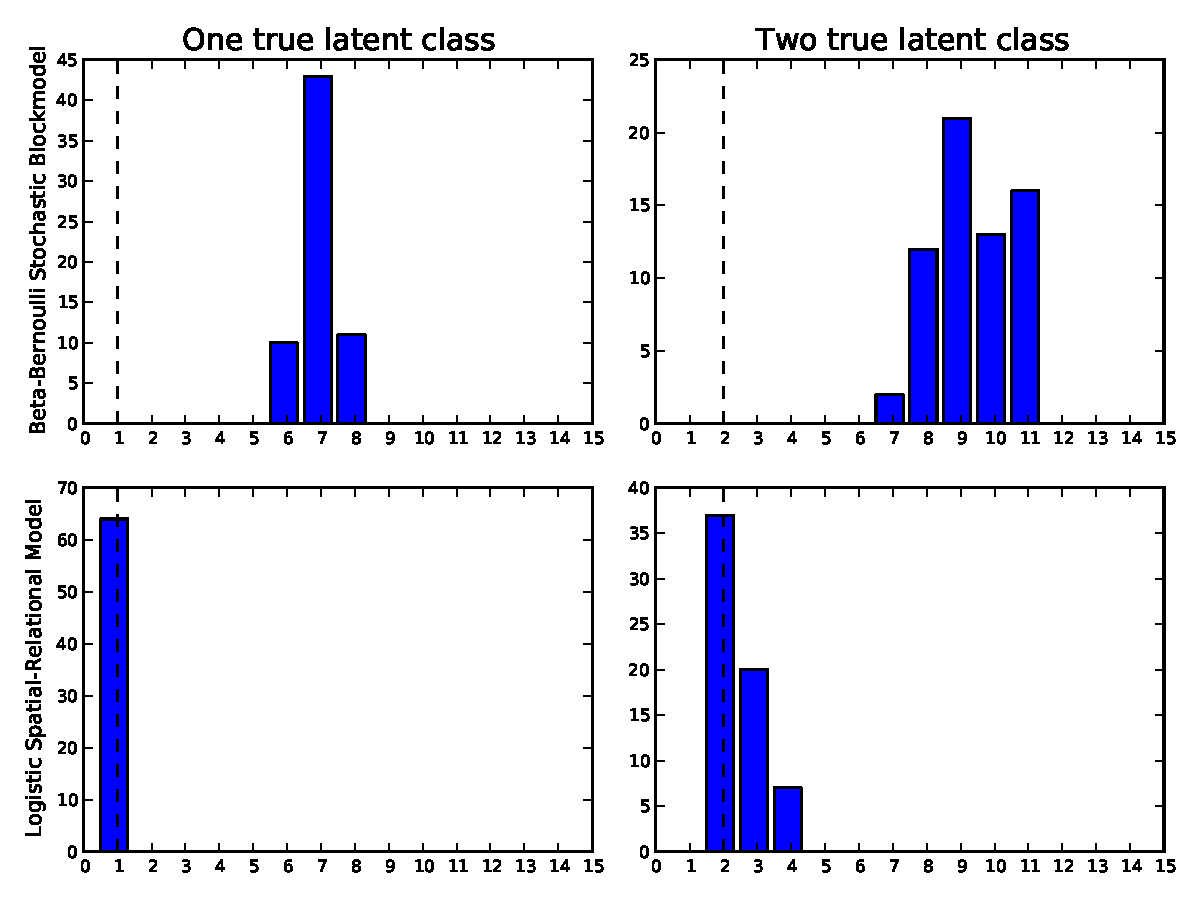
\includegraphics[width=0.5\textwidth]{comparison.pdf}
  \caption{Posterior distributions for the number of found latent classes. Synthetic datasets with spatially-localized connectivity and one (left) and t two (right) true latent classes were created. The regular beta-bernoulli infinite relational model (top) over-segements the data dramatically, whereas the spatial-relational model with the logistic-distance bernoulli likelihood recovers the true number of classes}
\end{figure}
  

\subsubsection{Arbitrary discriminative functions}
We can extend models of this type 

\begin{equation}
P(e_i, e_j) \sim F(g_{mn}(e_i, e_j))
\end{equation}

where $g_{mn}$ is an arbitrary link function $g$ defined per-latent
class -- if $e_i$ is of latent class $m$ and $e_J$ is of latent class
$n$, then the likelihood function $F$ is evaluated at $g_{mn}(e_i,
e_j)$ instead of a fixed parameter $\eta_{mn}$ in the classical
model. This allows an arbitrary discriminative function between
additional parameters of entities $e_i$ and $e_j$. That is, $g$ can be
defined on additional per-entity attributes, like spatial location.

We're principally interested in spatial models, so we associate with each
entity $e_i$ a location in space, and parameterize a per-latent-class
link function 
\todo{later}

\subsubsection{Infinite prior}
exchangability 
chinese restaurant process prior



\subsection{Likelihoods}
We evaluated a collection of link functions. 
Many of these are needed to map from $\mathbb{R}^+$ to some closed interval. 
TODO where do we talk about how this is like GLMs? 

Let $x_i$ and $x_j$ be the spatial locations of entities $e_i$ and $e_j$. $D(e_i, e_j$ is the euclidian distance between these two points. 
 
\subsubsection{Logistic Distance}
We use a binary observation for the relation (Bernoulli), and the $p$ is determined
on a per-class basis

prior on mu, lambda

\begin{figure}
  \centering 
  \begin{subfigure}[b]{0.4\textwidth}
    \includegraphics[height=1.5in]{logisticdistance.ai}
    \caption{Logistic-Distance Bernoulli Likelihood}
    \label{fig:gull}
  \end{subfigure}
  \begin{subfigure}[b]{0.4\textwidth}
    \includegraphics[height=1.5in]{exponentialdistancepoisson.ai}
    \caption{Exponential-Distance Poisson Likelihood}
    \label{fig:gull}
  \end{subfigure}

\end{figure}

This likeilihood model uses a logistic transform from distance to the
probability $p$ of a connection between two entities $e_i$ and
$e_j$. The latent class component parameters are the center of the
logistic $\mu_{mn}$ and the scale $\lambda_{mn}$. If the distance
between $e_i$ and $e_j$ is less than $\mu_{mn}$ then they are more
likely to be connected. To smooth out the likelihood, we scale the logistic
function by $p_{\textrm{min}}$ and $p_{\textrm{max}}$

So the generative model is
\[\mu_{ab} \sim \exp(\mu^{hp}) \]
\[\lambda{ab} \sim \exp(\lambda^{hp}) \]
\[p^* = \frac{1.0}{1.0 + \exp{\frac{(d(e_i, e_j) - \mu_{ab})}{\lambda_{mn}}}}\]
and then 
\[ r \sim \operatorname{Bernoulli}(p\cdot (p_{max} - p_{min}) + p_{min}) \]

\todo{example figure of parameterization, and notes}
We don't do hyperparameter inference on $p_{min}$ and $p_{max}$. 

\subsubsection{Normal Distance Fixed witdh}

\subsubsection{Exponential Distance Bernoulli}
\todo{Implement and test this model}


\subsubsection{Exponential Distance Poisson}
For distance-based models with count-based observations, we use an exponential 

\todo[inline]{Poisson is a pain because of linked mean/var}



\subsubsection{Exponential Distance Normal}


\subsubsection{Non-spatial, Conjugate likelihoods for comparison}
Beta Bernoulli
Gamma-Poisson

\subsection{Inference}

We use Markov-chain Monte Carlo techniques to sample from the posterior 
distribution of our model conditioned on the data. Inference is
performed over cluster assignments, the per-component latent parameters, 
and the per-relation, datatype-specific parameters. 


\subsubsection{Structural Inference}
Algorithm 8 from radford neal \autocite{Neal2000} for dirichlet process
inference. 


\subsubsection{Per-component parameters in nonconjugate case}
Slice sample on latent parameters \autocite{Neal2003}


\subsubsection{Hyperparameter Inferece}
Gridded gibbs sampling for hyperparameter inference
We set the grid by hand (empirical bayes)


\subsubsection{Annealing}
For many examples of the data here we perform annealing on the global likelihood during the burn-in period.  


\section{Results}

\subsection{Synthetic Data}
Show that traditional stochastic block model fails. 


The goal of the synthetic results is to show that we recover ground truth. 
1. where is the data from? 
2. how did we generate it? 


\subsection{Mouse Retina}

Dense serial electron microscopy of a $VOLUMNE$ in the mouse
retina by \autocite{Helmstaedter2013} yielded a listing of places where
neurons come into contact. There were $number$ cells originally, whcih
were refined through various classification schemes. We selected the
$950$ for which the location of the soma could be reconstruted from
the provided cell plots (soma locations were not provided by the
study's authors in machine-readble form).

The authors were unable to disambiguate actual ``synapses'' in the
full data set, but were able to measure the points of contact between
cells. Thus we don't have ``real'' synapses. We also don't have directionality. 

\begin{figure}
  \centering 
  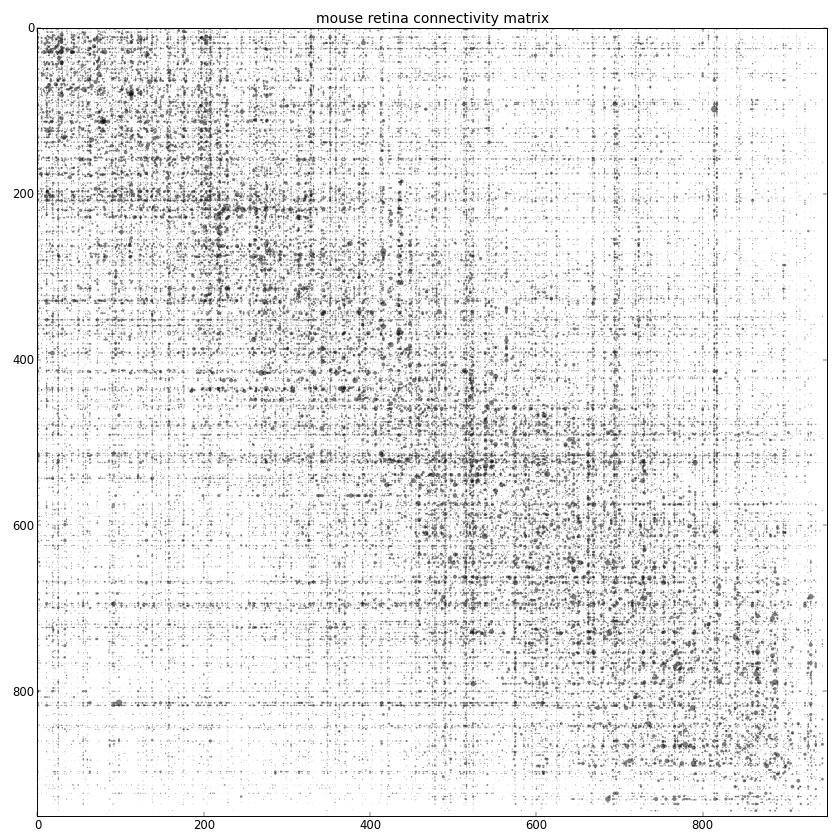
\includegraphics[width=0.5\textwidth]{mouseretina/adjmat.byz.png}
  \caption{Mouse connectome for the 950 cells with known soma positions, ordered by the position of the soma along the $z$ axis. The size of each point is proportional to the total area of contact between the cells.}
  \label{fig:mouseretina:adj}
\end{figure}

\subsubsection{Results}

\begin{figure}
  \centering 
  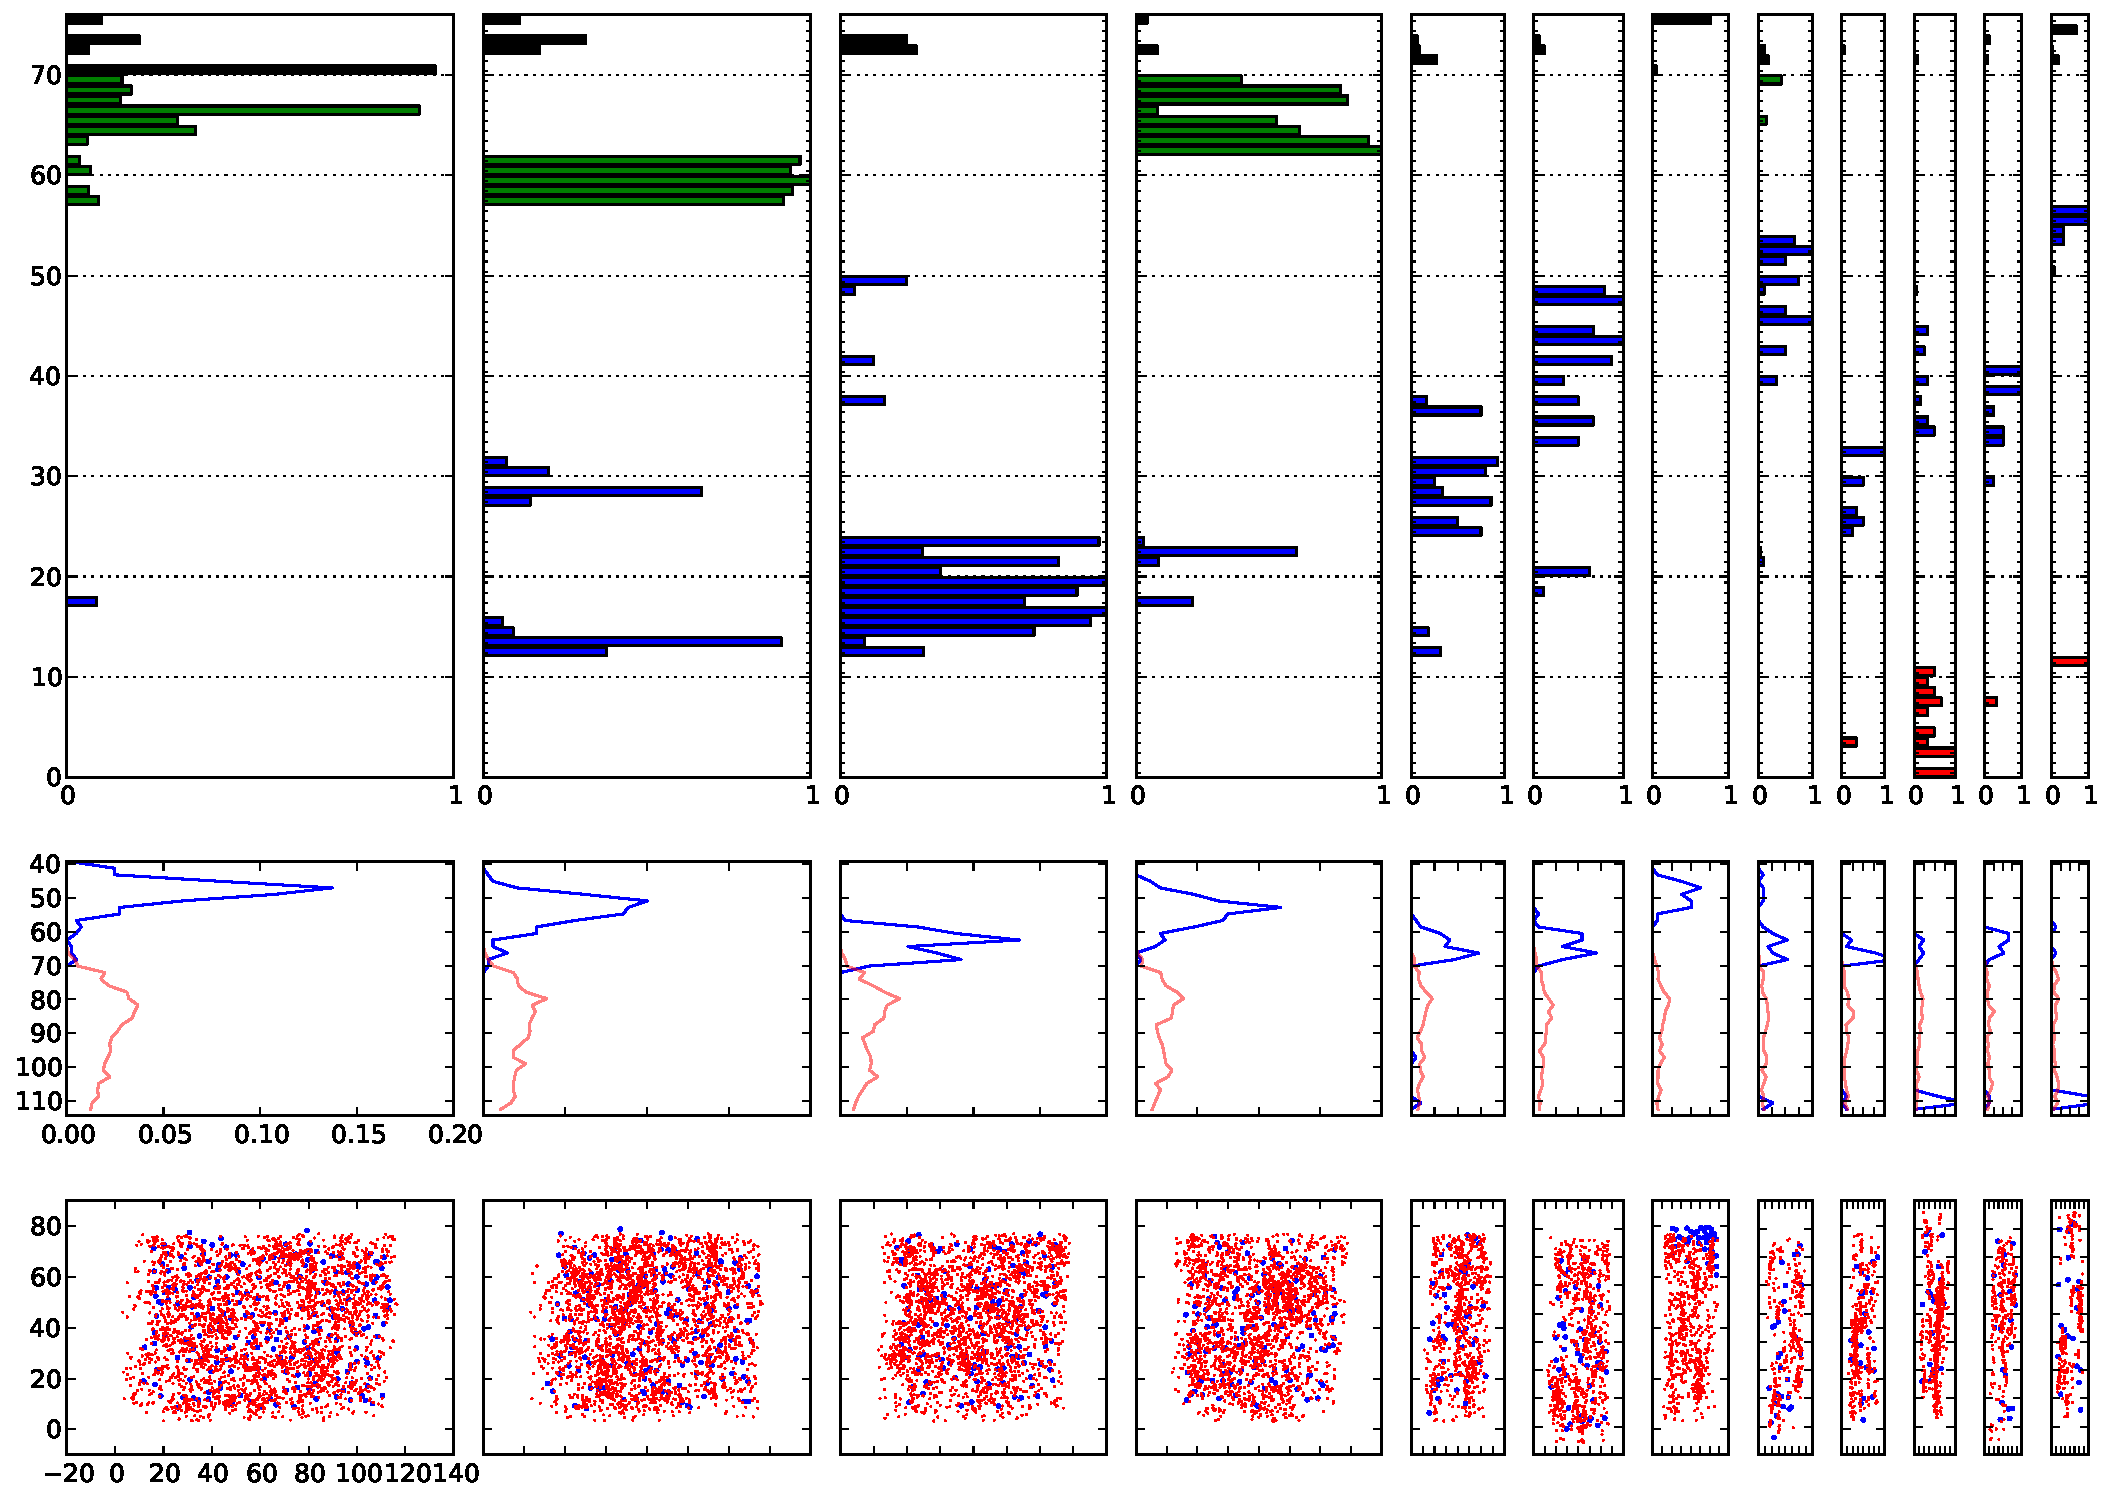
\includegraphics[width=\textwidth]{mouseretina/retina.1.0.ld.0.0.data-fixed_20_100-anneal_slow_400.0.clusters.pdf}
  \caption{Identified clusters from the mouse retina connectome using a Logistic-Distance-Bernoulli likelihood. Each column of plots is a cluster, wider plots for clusters with more cells. \textbf{first row} of plots compares the identified cluster to the experimenter-provided latent cell types, of which there were 74. Each bar is the fraction (between 0 and 1) of the cells of that type that are in this cluster. Note that the experimentors ordered their latent cell types, so cell type 60 is closer to 61 than 65 (see main text). Colors reflect the macro cell types (red = retinal ganglion cells, blue are amacrine, green are bipolar, and black are other. \textbf{Second row} is the spatial distribution of soma (blue) and synapses (red) for this cluster along a direction approximately normal to the retina surface. \textbf{Third row} is the spatial distribution of the soma (blue dots) and synapses (red dots) in this cluster, across the retina surface.}
  \label{fig:mouseretina:clusters}
\end{figure}

\begin{figure}
  \centering 
  \begin{subfigure}[b]{0.46\textwidth}
    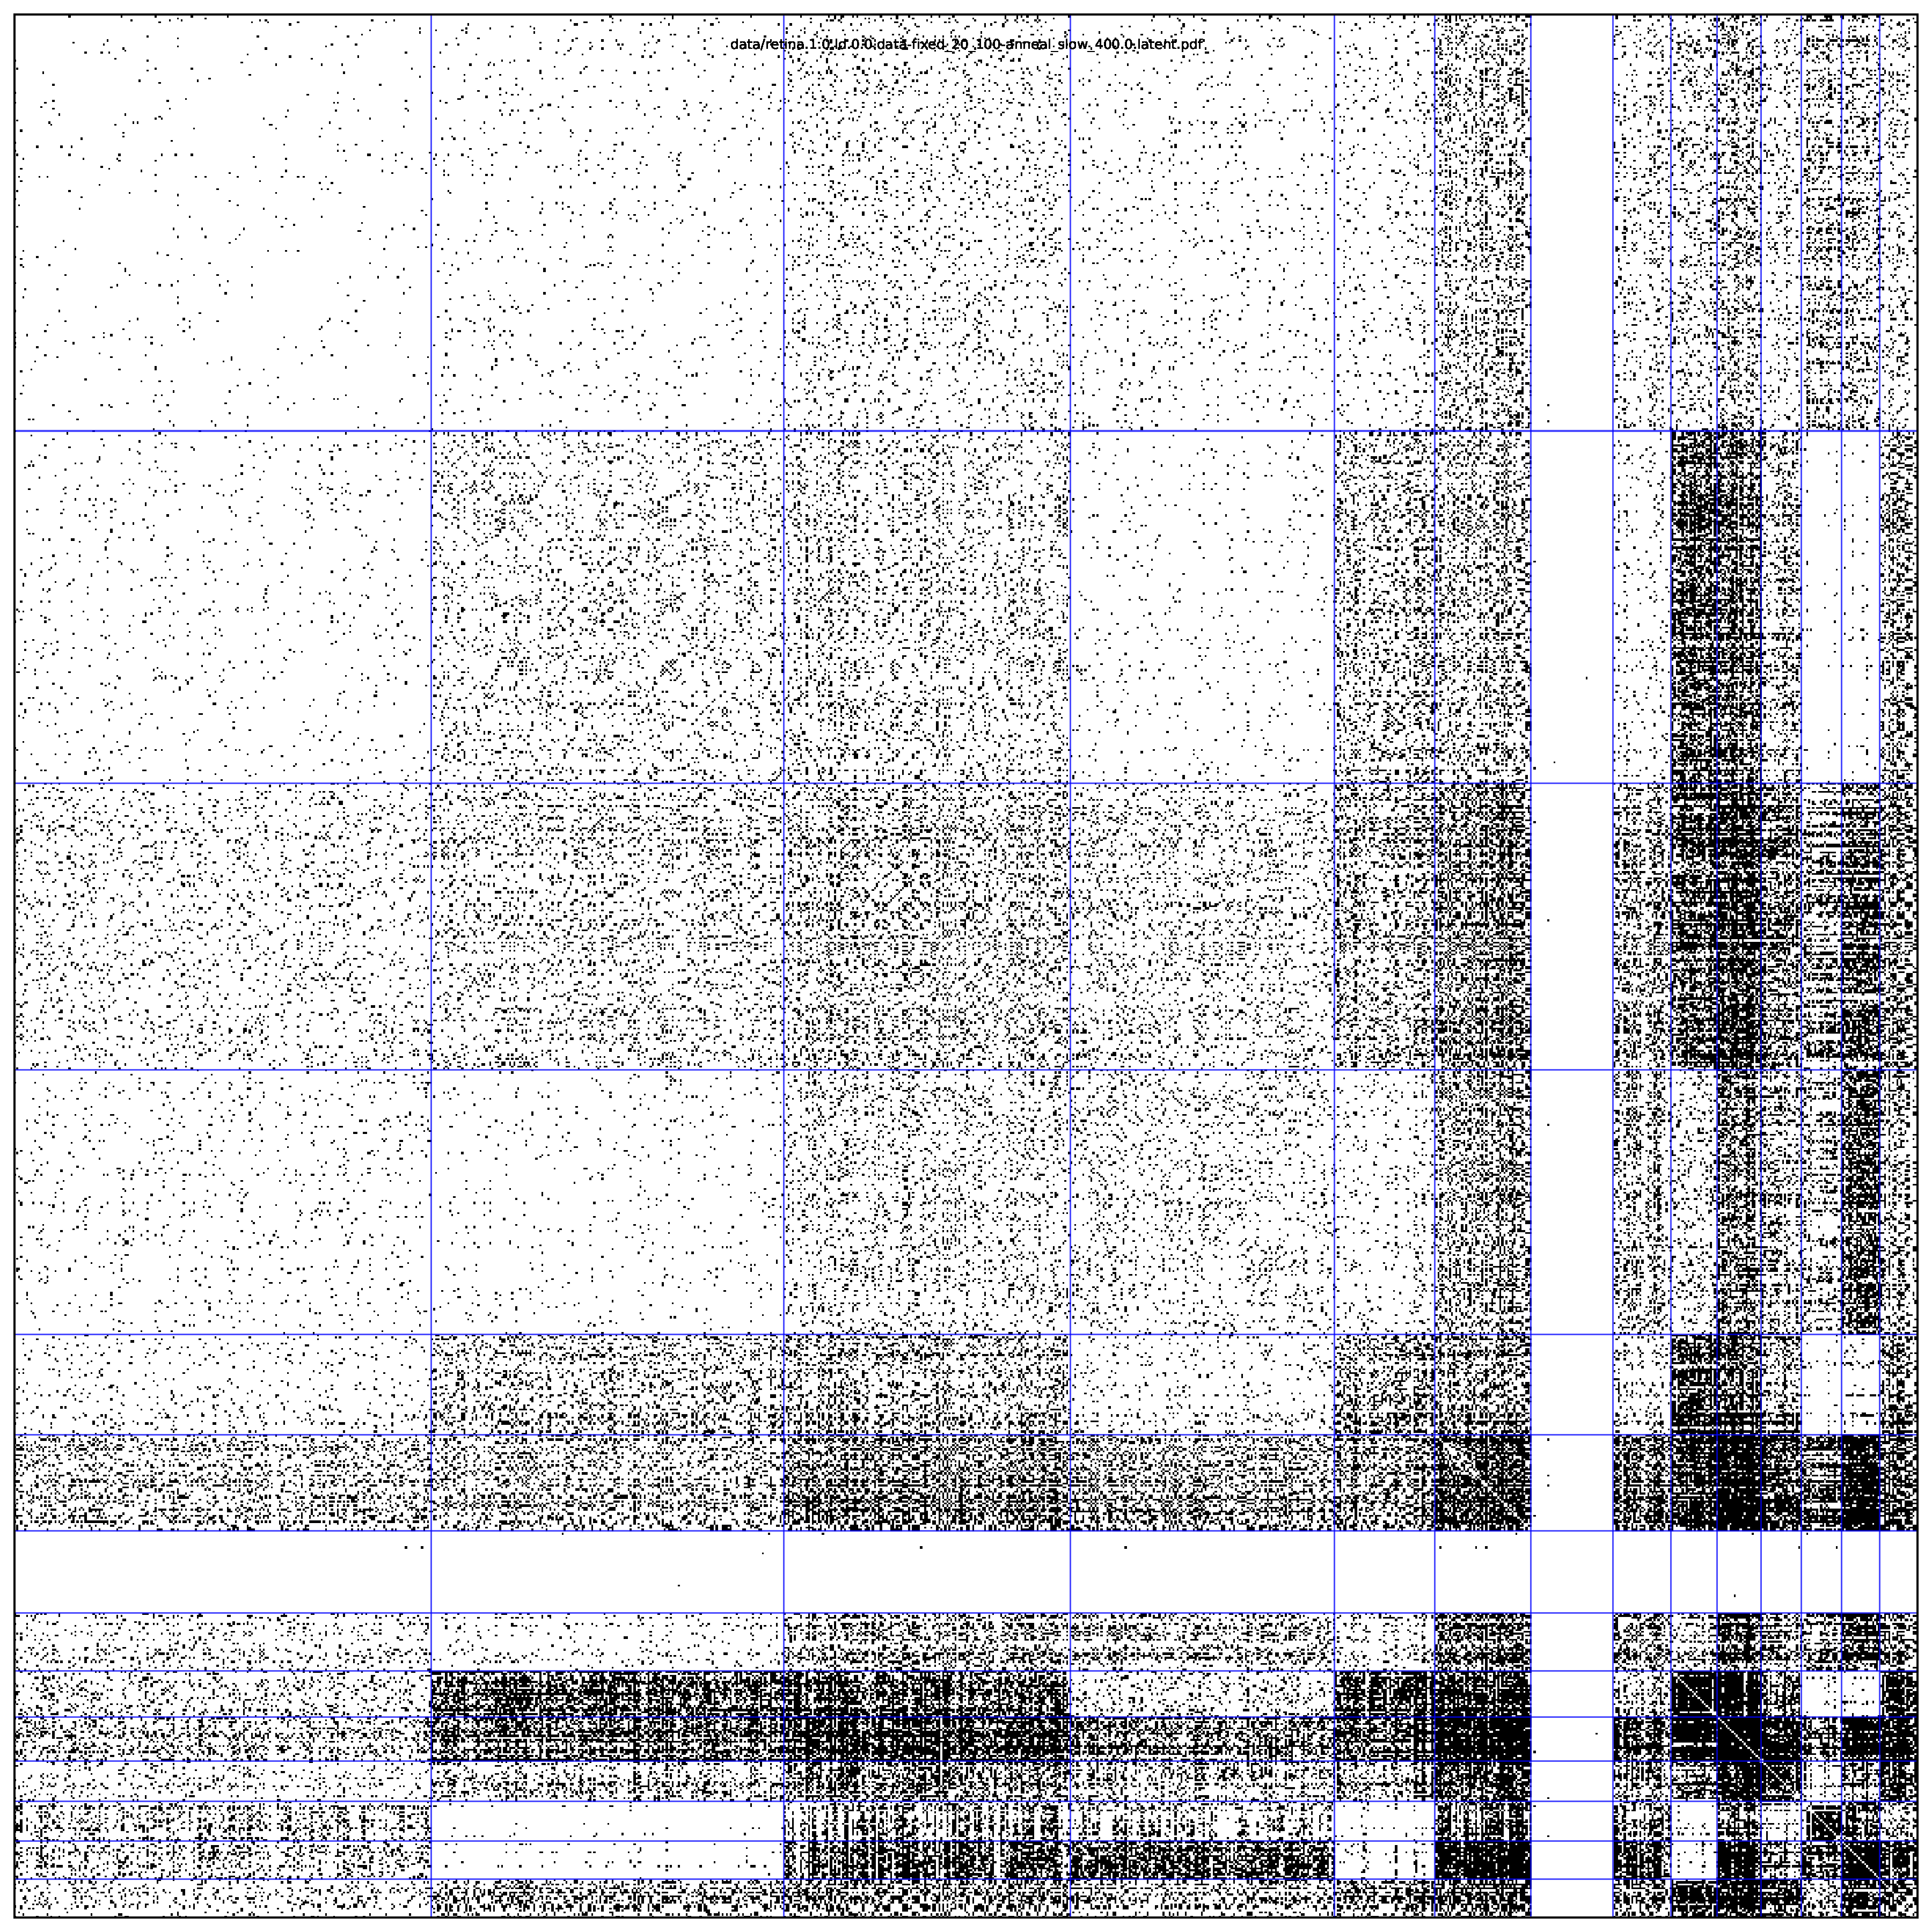
\includegraphics[width=\textwidth, page=1]{mouseretina/retina.1.0.ld.0.0.data-fixed_20_100-anneal_slow_400.0.latent.pdf}
    \caption{Clustered latent connectivity matrix.}
    \label{fig:gull}
  \end{subfigure}
  \begin{subfigure}[b]{0.46\textwidth}
    \includegraphics[width=\textwidth, page=2]{mouseretina/retina.1.0.ld.0.0.data-fixed_20_100-anneal_slow_400.0.latent.pdf}
    \caption{Latent cluster parameters. }
    \label{fig:gull}
  \end{subfigure}
  \caption{Latent structure for mouse retina connectome clusters above. The latent cluster parameters in (b.) show (blue) the empirical distribution of connectivity for this cluster as a function of distance, and (red) the fit logistic curve. The vertical black line is the value of $\mu$.}
  \label{fig:mouseretina:latent}
\end{figure}

\subsection{C. elegans}

The connectome of the nematode Caenorhabditis elegans was traced by
hand from serial electron micrographs from Sidney Brenner's laboratory
in 1986 \autocite{White1986}. \textit{C. elegans} exhibits extremely
stereotypic neural development, with each hermaphrodite animal having
exactly 302 neurons, and the synaptic connectivity being 75\%
identical \todo{where did this number come from} across animals. Here we
examine 279 nonpharyngeal neurons with 6393 chemical synapes and 890 electrical junctions originally cleaned up in \autocite{Chen2006}. The adjacency matrix is shown in figure~\ref{fig:celegans:adj}  

\begin{figure}
  \centering 
  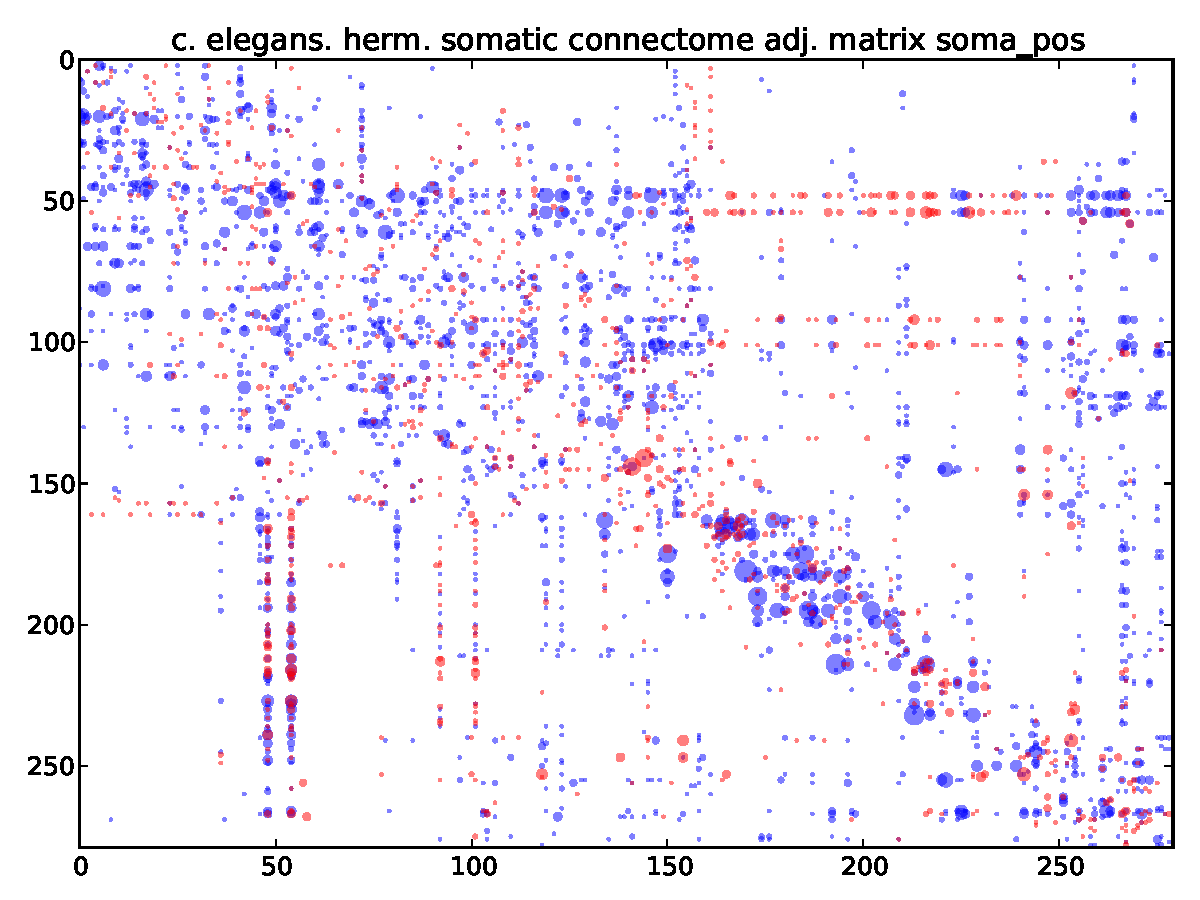
\includegraphics[width=0.5\textwidth]{celegans/data.pos.pdf}
  \caption{Connectome for the 279 nonpharyngeal cells in \textit{c. elegans}. Cells are ordered by their position along the body axis. Blue dots are chemical synapses, red dots are electrical synapses, and the area of each dot is equivalent to the number of synaptic contacts between the cells. Note that the chemical synapses (blue) are directional, thus the red dots form a symmetric matrix}
  \label{fig:celegans:adj}
\end{figure}


The structure of the \textit{c. elegans} nervous system differs considerably 
from the primary sensory connectomes we examined: 

\begin{itemize}
\item Lots of ganglia with global projections
\item Many of Brenner's originally-identified cell types contain only two member cells, one on each side of the animal. 
\item We have both electrical and chemical synapses, where the chemical synapses are directional. 
\item Our position data only indicates the position along the body axis (on the interval $[0, 1]$. 
\end{itemize}

The neurons can be broadly classified into ``sensory'', ``motor'', and
``interneurons''. In addition, there are several broad classes of both
sensory and motor neurons containing up to twelve cells. Figure ~\ref{fig:celegans:classestruth} shows the locations the cells of the biggest classes. Note the anterior concentration of sensory and internurons in contrast to the broad spatial distribution of the motor neurons. 

\begin{figure}
  \centering 
  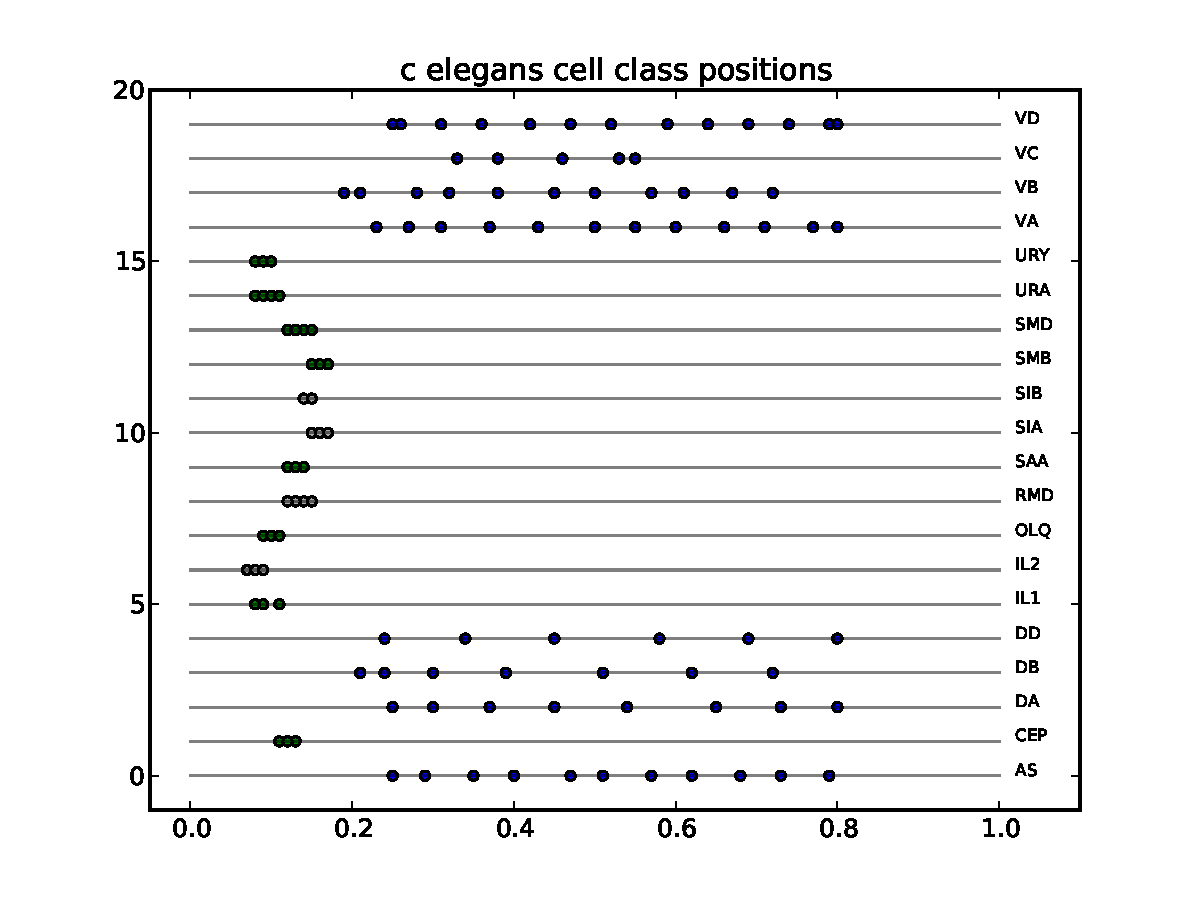
\includegraphics[width=0.7\textwidth]{celegans/class.positions.pdf}
  \caption{Positions of \textit{C. elegans} neurons grouped by cell type along the anterior-posterior axis. The cell type is listed to the right. Blue cells are motor neurons, green are sensory, and grey are interneurons. }
  \label{fig:celegans:classestruth}
\end{figure}

\subsubsection{Results}
We model \textit{C. elegans} using two $T1\times T1$ binary relations, one for the chemical synapses and one for the electrical synapses. Two cells are connected if they have at least one synapse between them, giving rise to a binary matrix for each synapse type. We see the results of two likelihood models in figure~\ref{fig:celegans:clusters}. The logistic-distance Bernoulli likelihood segements the sensory and interneurons from the spatially-distributed motor neurons, whereas the normal-distance fixed-width likelihood \todo{Write about this; adopt consistent naming} creates an odd collection of clusters. 



\begin{figure}
  \centering 
  \begin{subfigure}[b]{0.42\textwidth}
    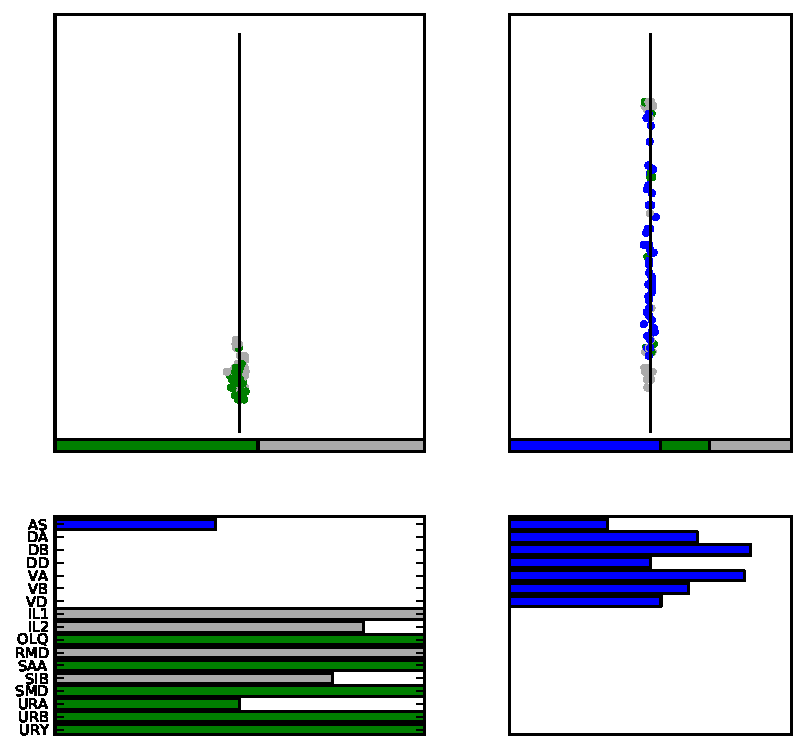
\includegraphics[width=\textwidth]{celegans/celegans.2r.ld.00.data-fixed_100_200-anneal_slow_400.0.clusters.pdf}
    \caption{Logistic-Distance Bernoulli}
    \label{fig:celegans:clusters:ld}
  \end{subfigure}
  \begin{subfigure}[b]{0.47\textwidth}
    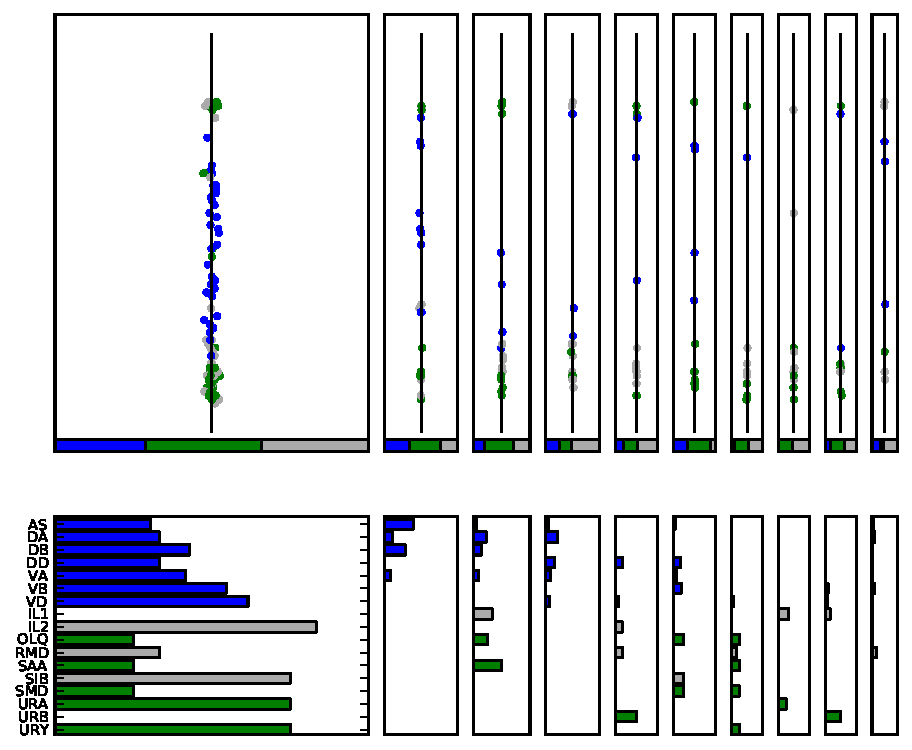
\includegraphics[width=\textwidth]{celegans/celegans.2r.ndfw.00.data-fixed_100_200-anneal_slow_400.0.clusters.pdf}
    \caption{Normal-Distance Fixed-Width}
    \label{fig:celegans:clusters:ndfw}
  \end{subfigure}
  \caption{C. elegans clusters for two different likelihoods, showing the clustering of the largest classically-known cell types. Green cells are sensory, grey are interneurons, and blue are motor neurons. The top row shows the cells in the cluster and where they are spatially; the bottom shows cluster purity. }
  \label{fig:celegans:clusters}
\end{figure}

\todo[inline]{Should we try to include the neuromuscular and sensory junctions? The data exists from wormatlas.org}

\todo[inline]{should we use the exponentail-distance-count likelihood?} 

\todo[inline]{Better understanding of how we model ganglia-like structures}
\subsection{Drosophila optic medulla}
Serial electron microscopy was used to reconstruct several columns from the Drosophila optic medulla \autocite{Takemura2013}. Experimenters were able to measure the physical location of the pre- and post-synaptic side of each synapse in the neuropil, and thus the directionality. The neural cell bodies in the cortex surround the neuropil and were not measured due to technique limitations \autocite{MeinertzhagenPersonalComm}, thus we don't know the spatial location of the soma. 

\begin{figure}
  \centering 
  \begin{subfigure}[b]{0.55\textwidth}
    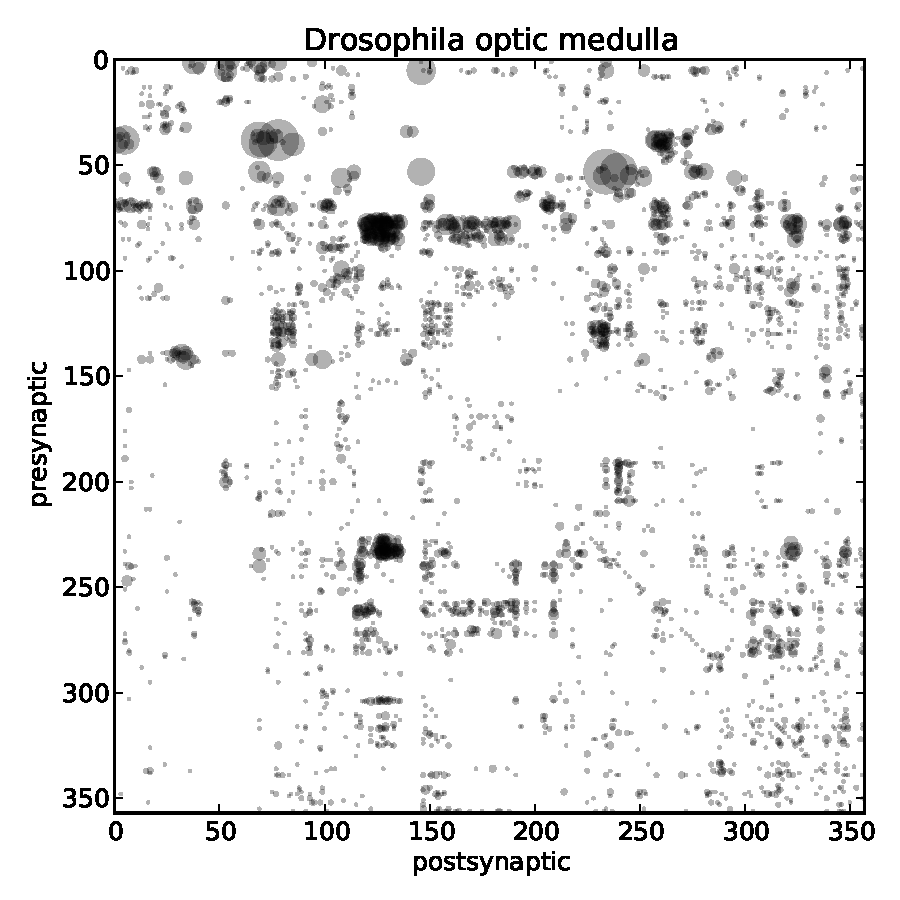
\includegraphics[width=\textwidth]{drosophila/adj_comp.pdf}
    \caption{Drosophila optic medulla connectome}
    \label{fig:drosophila:connectome}
  \end{subfigure}
  \begin{subfigure}[b]{0.4\textwidth}
    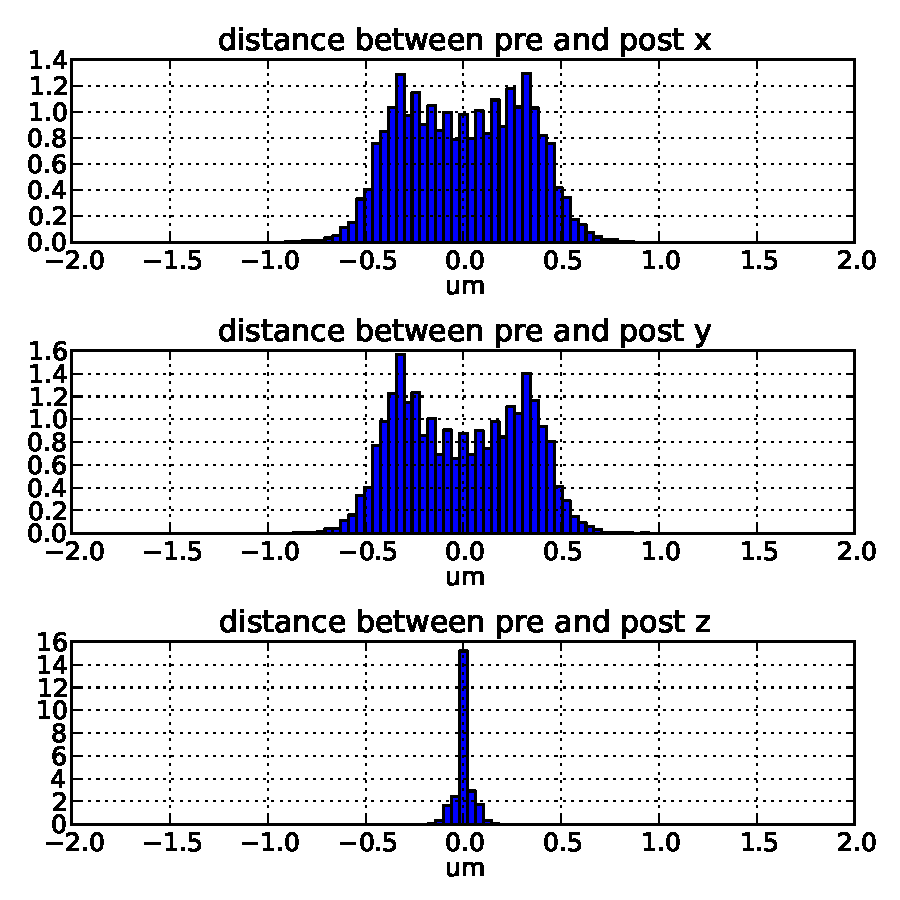
\includegraphics[width=\textwidth]{drosophila/pre_post_dist_hist.pdf}
    \caption{Pre and post-synaptic distance}
    \label{fig:drosophila:distprepost}
  \end{subfigure}
  \caption{a.) Connectome for the 357 cells in \textit{drosophila} medulla. Cells are ordered by the order they appear in the data file. Dot area is proportional to the number of synapses; data are directional. b.) Histogram of spatial distance between pre- and post-synaptic sites.}
  \label{fig:drosophila_adj}
\end{figure}

\subsubsection{Results}

From the provided spreadsheet of synapses we extract all synapses for cells with non-numeric IDs (357). We reduced the location of every synapse to the average of its pre and post-synaptic sites, as the average distance is small (figure~\ref{fig:drosophila:distprepost}). For a given postsynaptic cell, we average the spatial location of all of its postsynaptic sites, and assign this point as the cell's location. The resulting clusters from using the exponential-distance-Poisson model with synapse count observations is in figure~\ref{fig:drosophila:clusters_edp}. The clusterings are not obvious, and don't reflect any particular clean division of their existing labeled subtypes, although the block structure appears pretty solid. 

Next steps are:

\begin{itemize}
  \item Is the centroid of the presynaptic inputs the best point to use for the cell's ``distance'' calculations ? 
  \item I've tried both EDP and LD models for count and binary data respectively, without any obvious benefits
  \item How well do we really understand this system? My understanding both of the neuroanatomy and the data acquisition process for the mouse retina really guided my modelling efforts. I don't have that here, and need to read \autocite{Fischbach1989} to understand cell types. 
  \item Did the experimenters measure just a ``single'' column completely and then whatever happened to be in nearby columns that connected to this focus column? If so, we have complete observation data for only one microcircuit. 
    \item Are we sure this isn't just the result of some preprocessing bug? I need to run synthetic data through this pipeline. 
      
    \end{itemize}
    
\begin{figure}
  \centering
  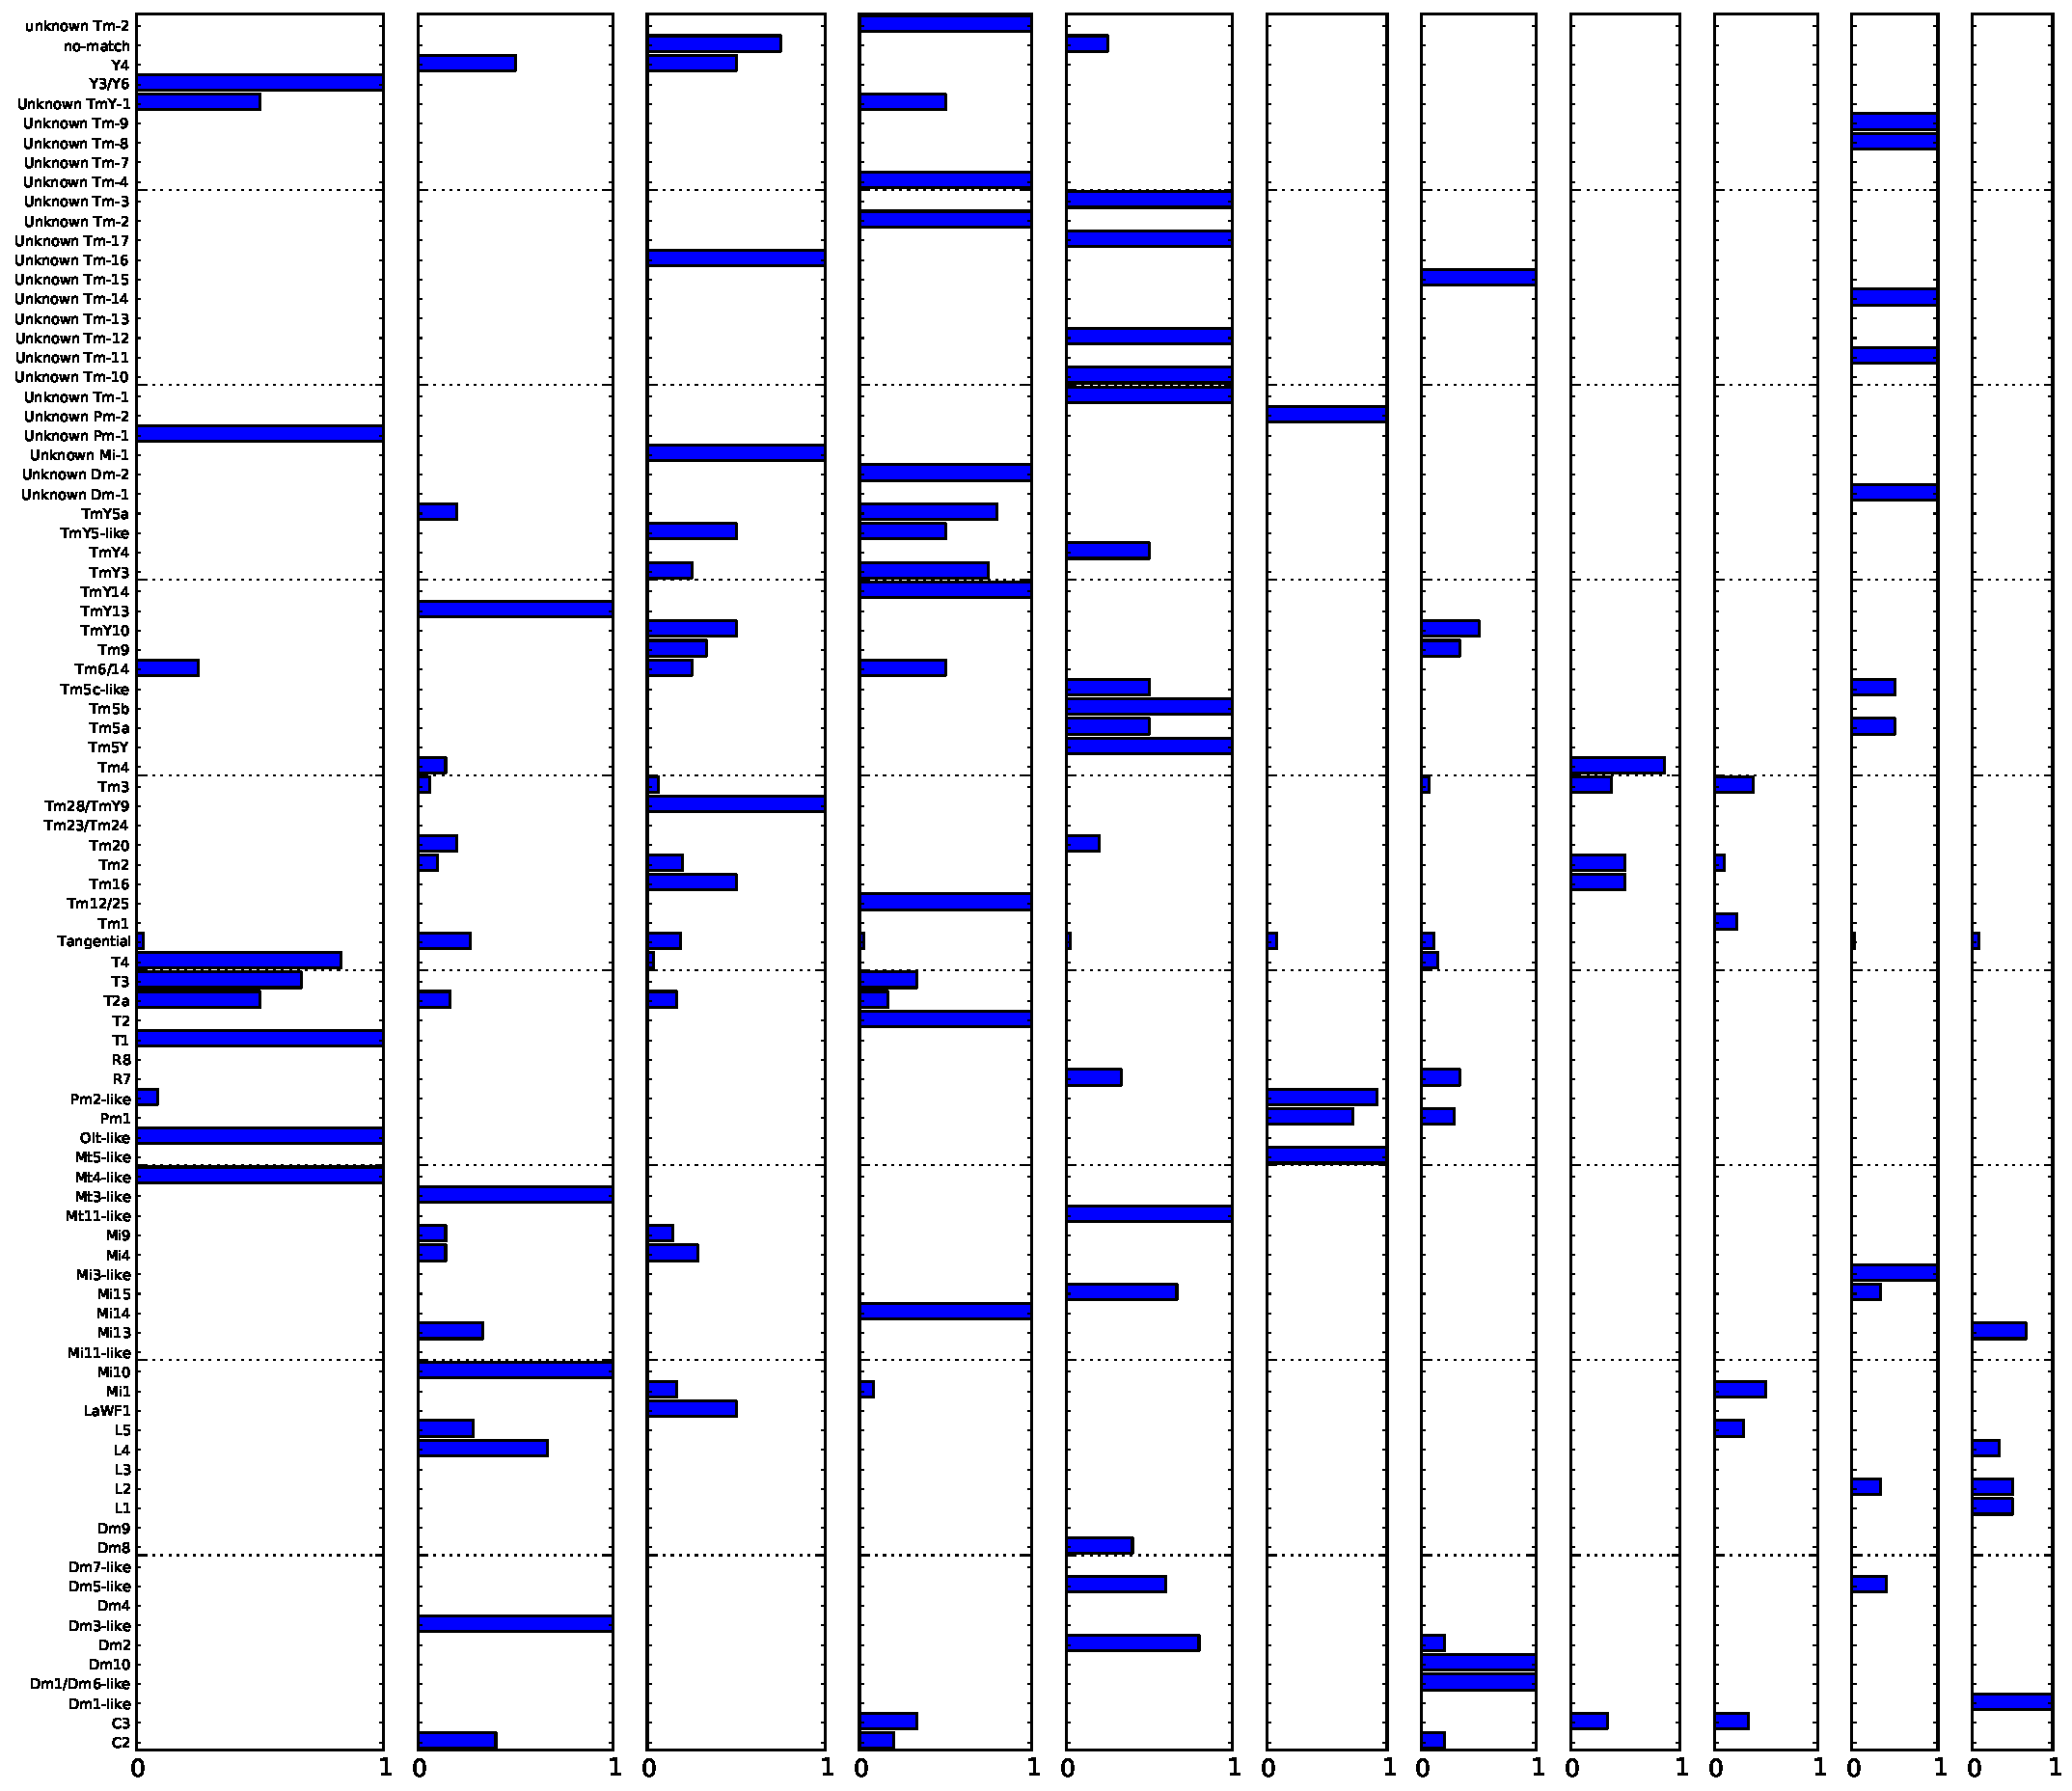
\includegraphics[width=\textwidth]{drosophila/drosophila.edp.data-fixed_100_200-anneal_slow_400.0.clusters.pdf}
  \caption{Discovered latent clusters for Drosophla optic medulla via Exponential-Distance Poisson likelihood.}
  \label{fig:drosophila:clusters_edp}
\end{figure}

\begin{figure}
  \centering
  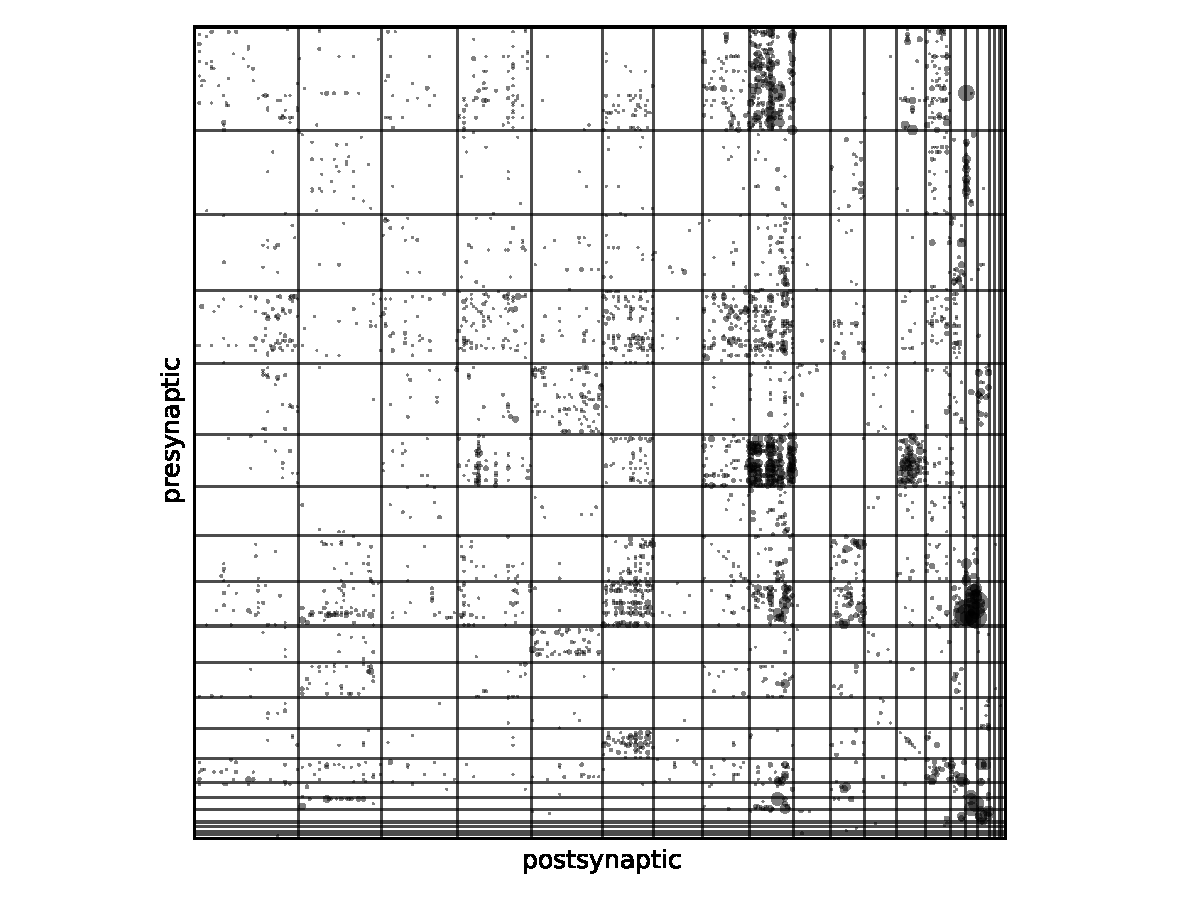
\includegraphics[width=\textwidth]{drosophila/drosophila.edp.data-fixed_100_200-anneal_slow_400.0.latent.pdf}
  \caption{Clustered connectivity matrix for Drosophila optic medulla via Exponential-Distance Poisson likelihood.}
  \label{fig:drosophila:latent_edp}
\end{figure}

\subsection{MOS 6502}

Hobbiest groups seeking to preserve historical microprocessors have
measured the ``connectomes'' of silicon integrated circuits. This
process involves obtaining classic chips, removing the casing
chemically, and then taking multi-gigapixel visible-light micrographs
of the silicon layers contained within. Then, a partially automated
process is used to read out the silicon polygons and reconstruct the
processor circuit contained within. The results are quite impressive,
with groups having successfully measured the original MOS6502 (Found
in the Apple I), and then used this ``connectome'' to perform
cycle-accruate simulation.


\begin{figure}
  \centering 
  \begin{subfigure}[b]{0.43\textwidth}
    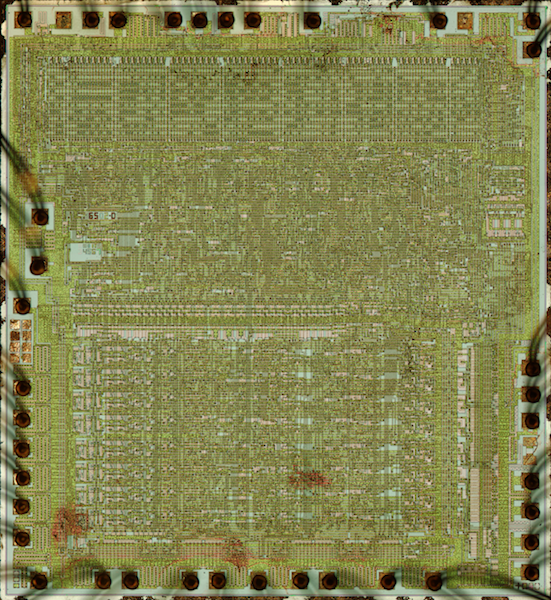
\includegraphics[width=\textwidth]{mos6502/6502_shrunk.png}
    \caption{MOS 6502 die}
    \label{fig:mos6502:die}
  \end{subfigure}
  \begin{subfigure}[b]{0.50\textwidth}
    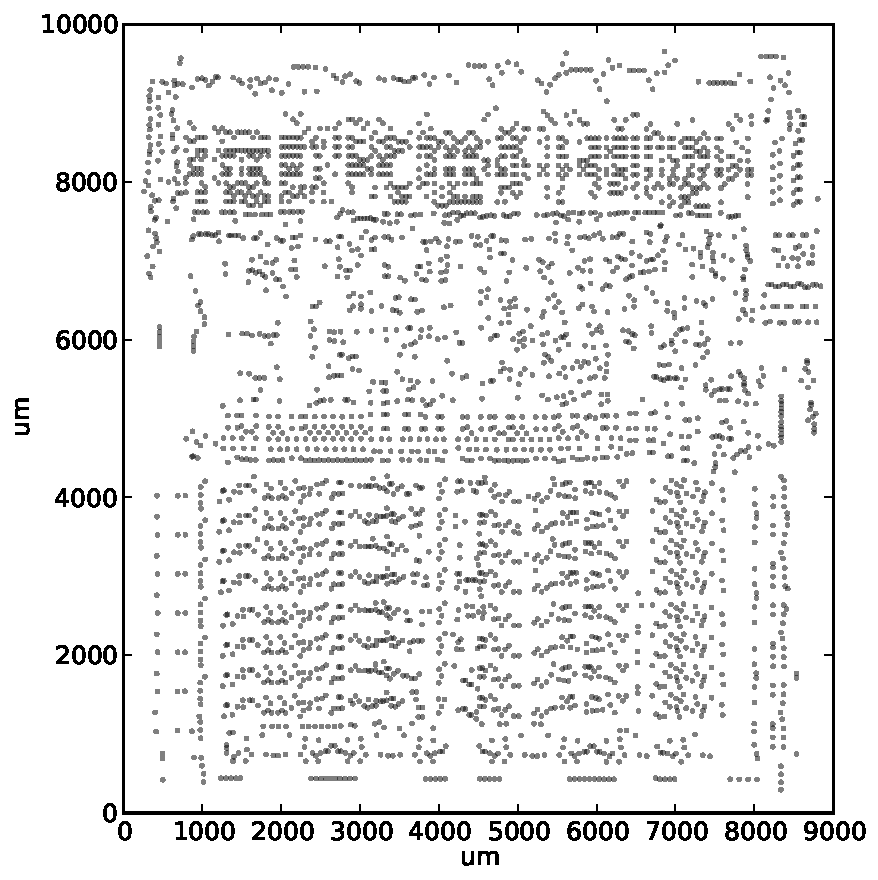
\includegraphics[width=\textwidth]{mos6502/transistors.pdf}
    \caption{Identified transistor locations}
    \label{fig:mos6502:transistors}
  \end{subfigure}
  \begin{subfigure}[b]{0.7\textwidth}
    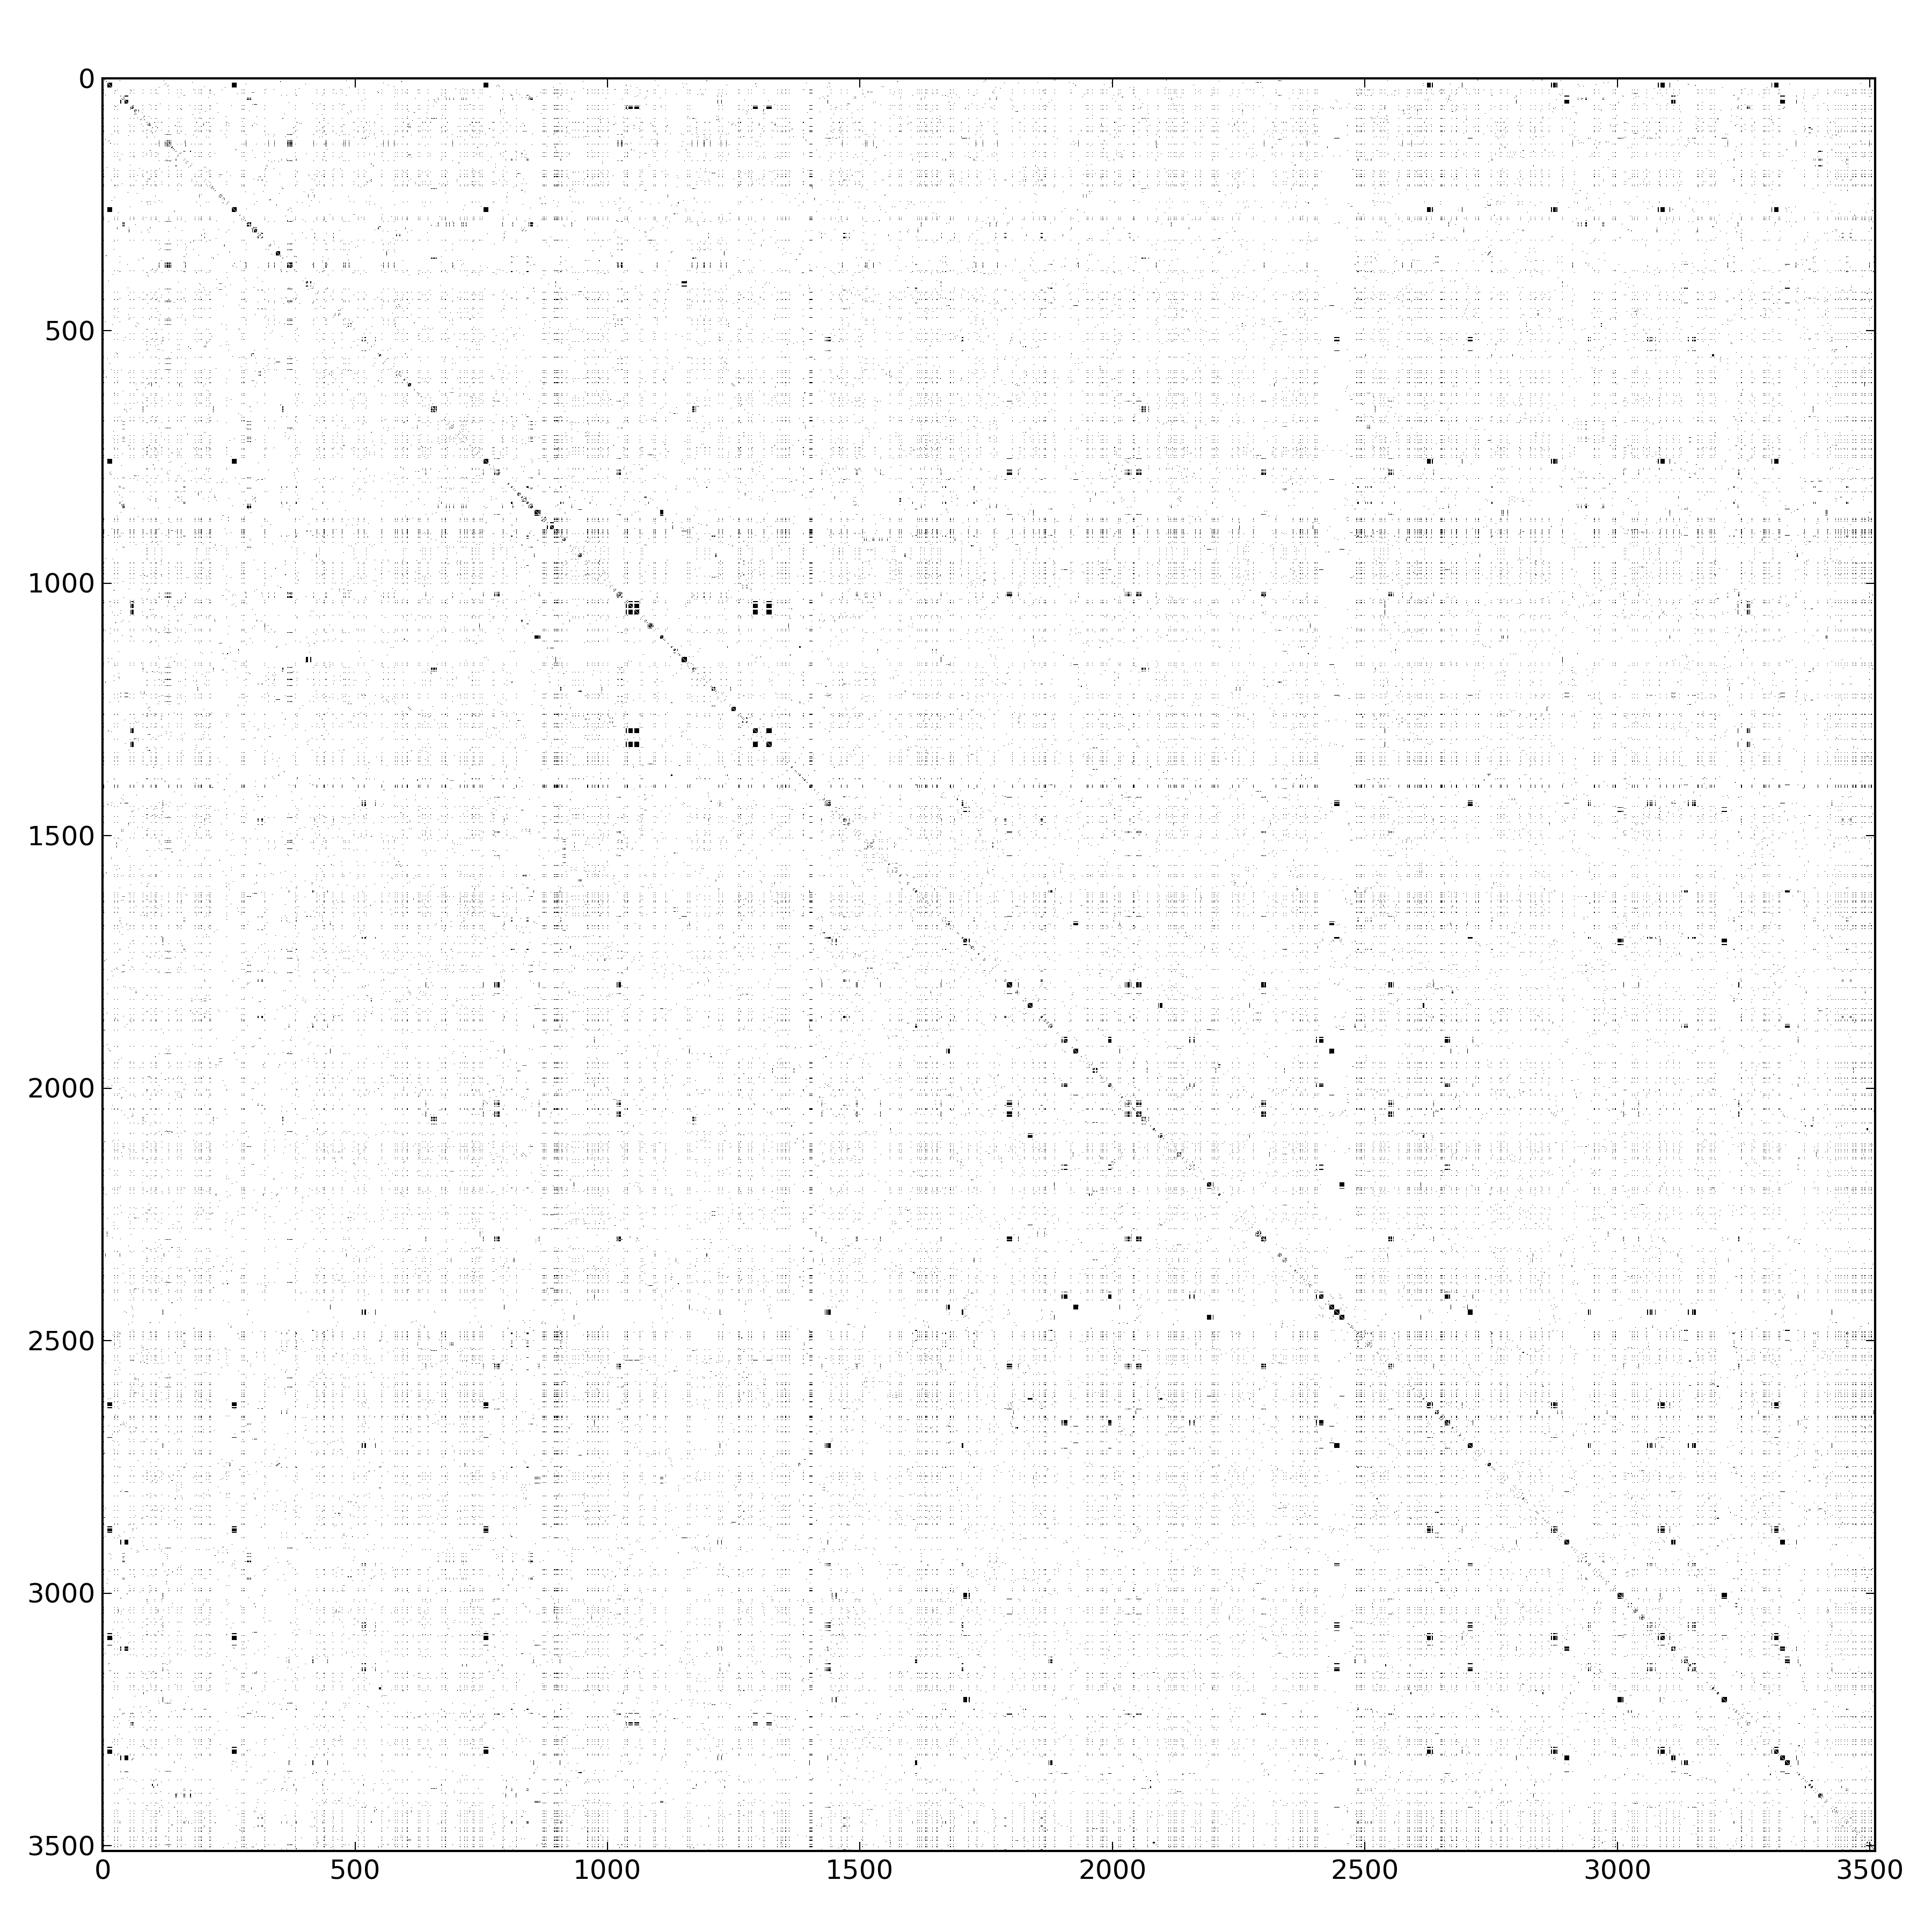
\includegraphics[width=\textwidth]{mos6502/all.adj.png}
    \caption{Adjacency matrix for entire IC}
    \label{fig:mos6502:adj}
  \end{subfigure}
  \caption{}
  \label{fig:mos6502:adjj}
\end{figure}

\subsubsection{Results}

We extracted this data at the per-transistor level from the online
github project, resulting in $NUMBER$ transistors. Each MOS transistor
has three terminals: $g$, $c_1$, and $c2$. The resulting data is then
a bipartate graph between the terminals of the transistors and various
voltage ``nodes'', the wires that connect them. At the physical level
electronic circuits are fundamentally undirected, and all terminals
connected to a node will be at the same voltage. Ideally we'd be
operating at a higher level of abstraction with digital elements (logic gates,
registers) with more clearly-defined inputs and outputs, but this
was the only data set available. 

For our encoding, the entities are transistors, and the relation is
true if any terminal of the transistor connects to any terminal of any
other transistor. This results in an incredibly densely-connected
graph, as almost all transistors are connected to very common nodes
like ``power'', ``ground'', and the global clock, which we remove
prior to analysis. We look at two subsets of the total chip, the
instruction decoding region and the region consisting of the ``X'',
``Y'', and ``S'' registers.

\begin{figure}[h]
\centering
\begin{subfigure}[b]{0.43\textwidth}
  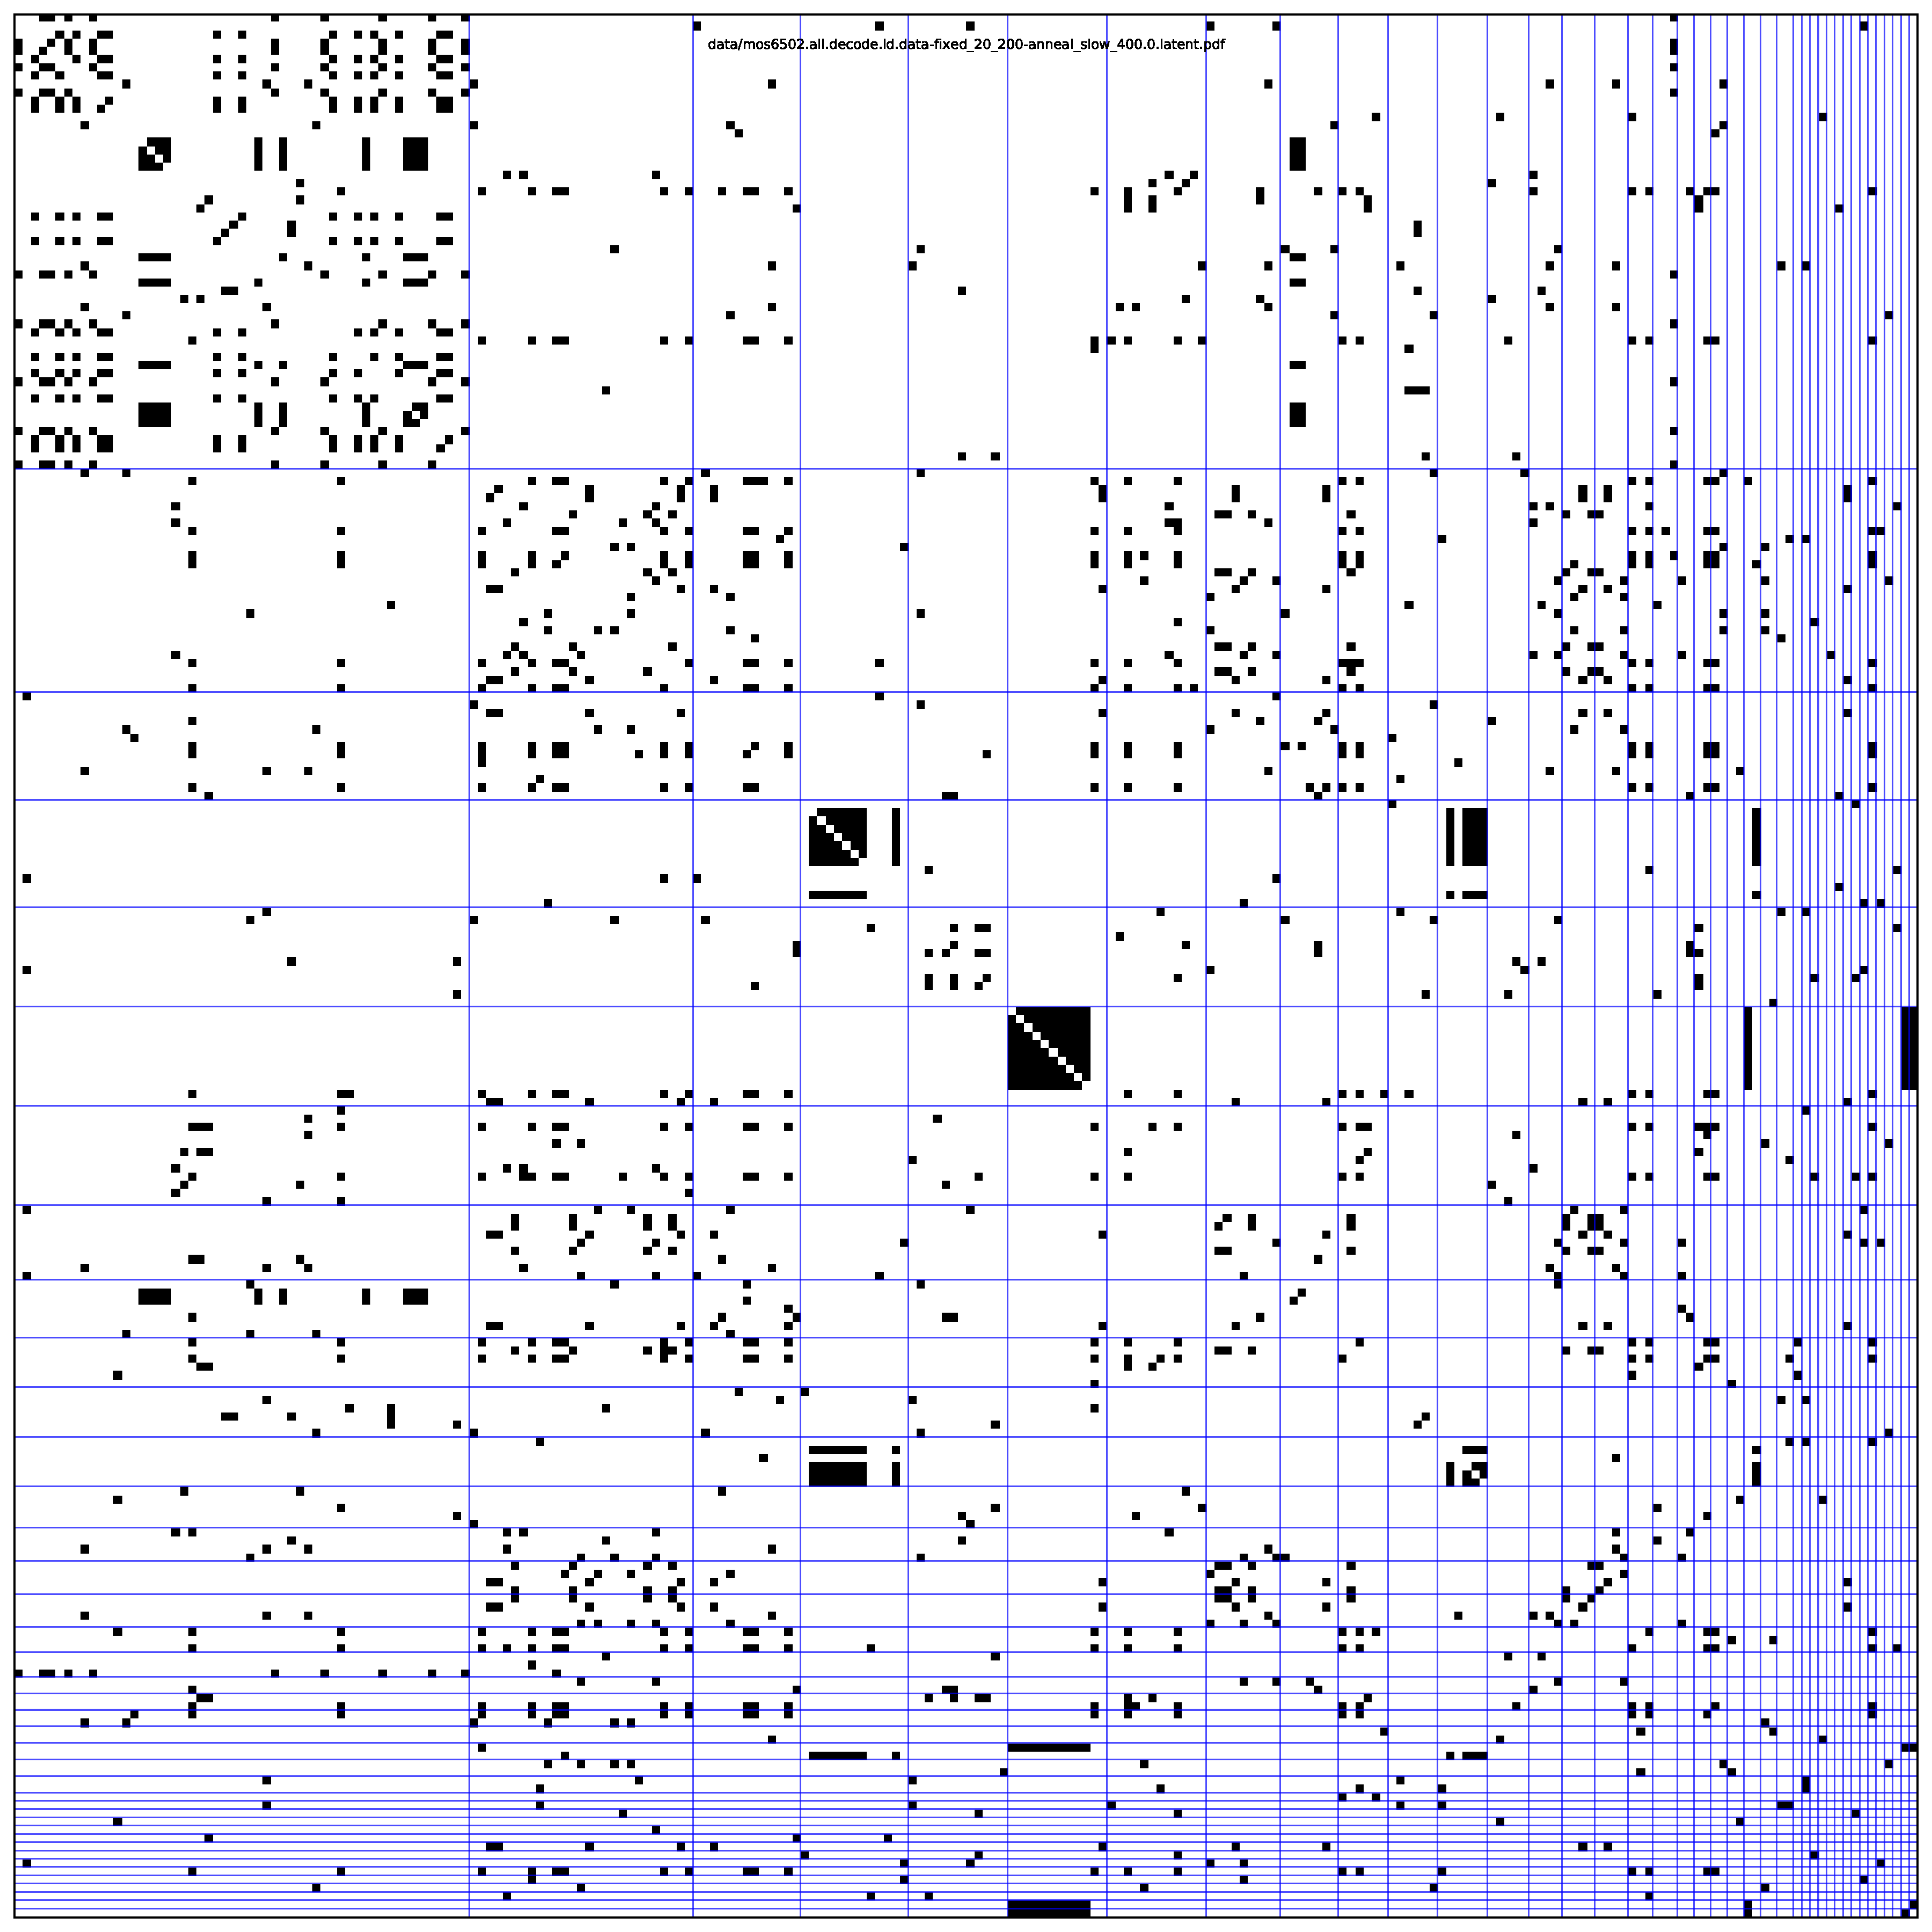
\includegraphics[width=\textwidth]{mos6502/mos6502.all.decode.ld.data-fixed_20_200-anneal_slow_400.0.latent.pdf}
  \caption{MOS 6502 Instruction Decode Latent}
\end{subfigure}
  
\begin{subfigure}[b]{0.43\textwidth}
  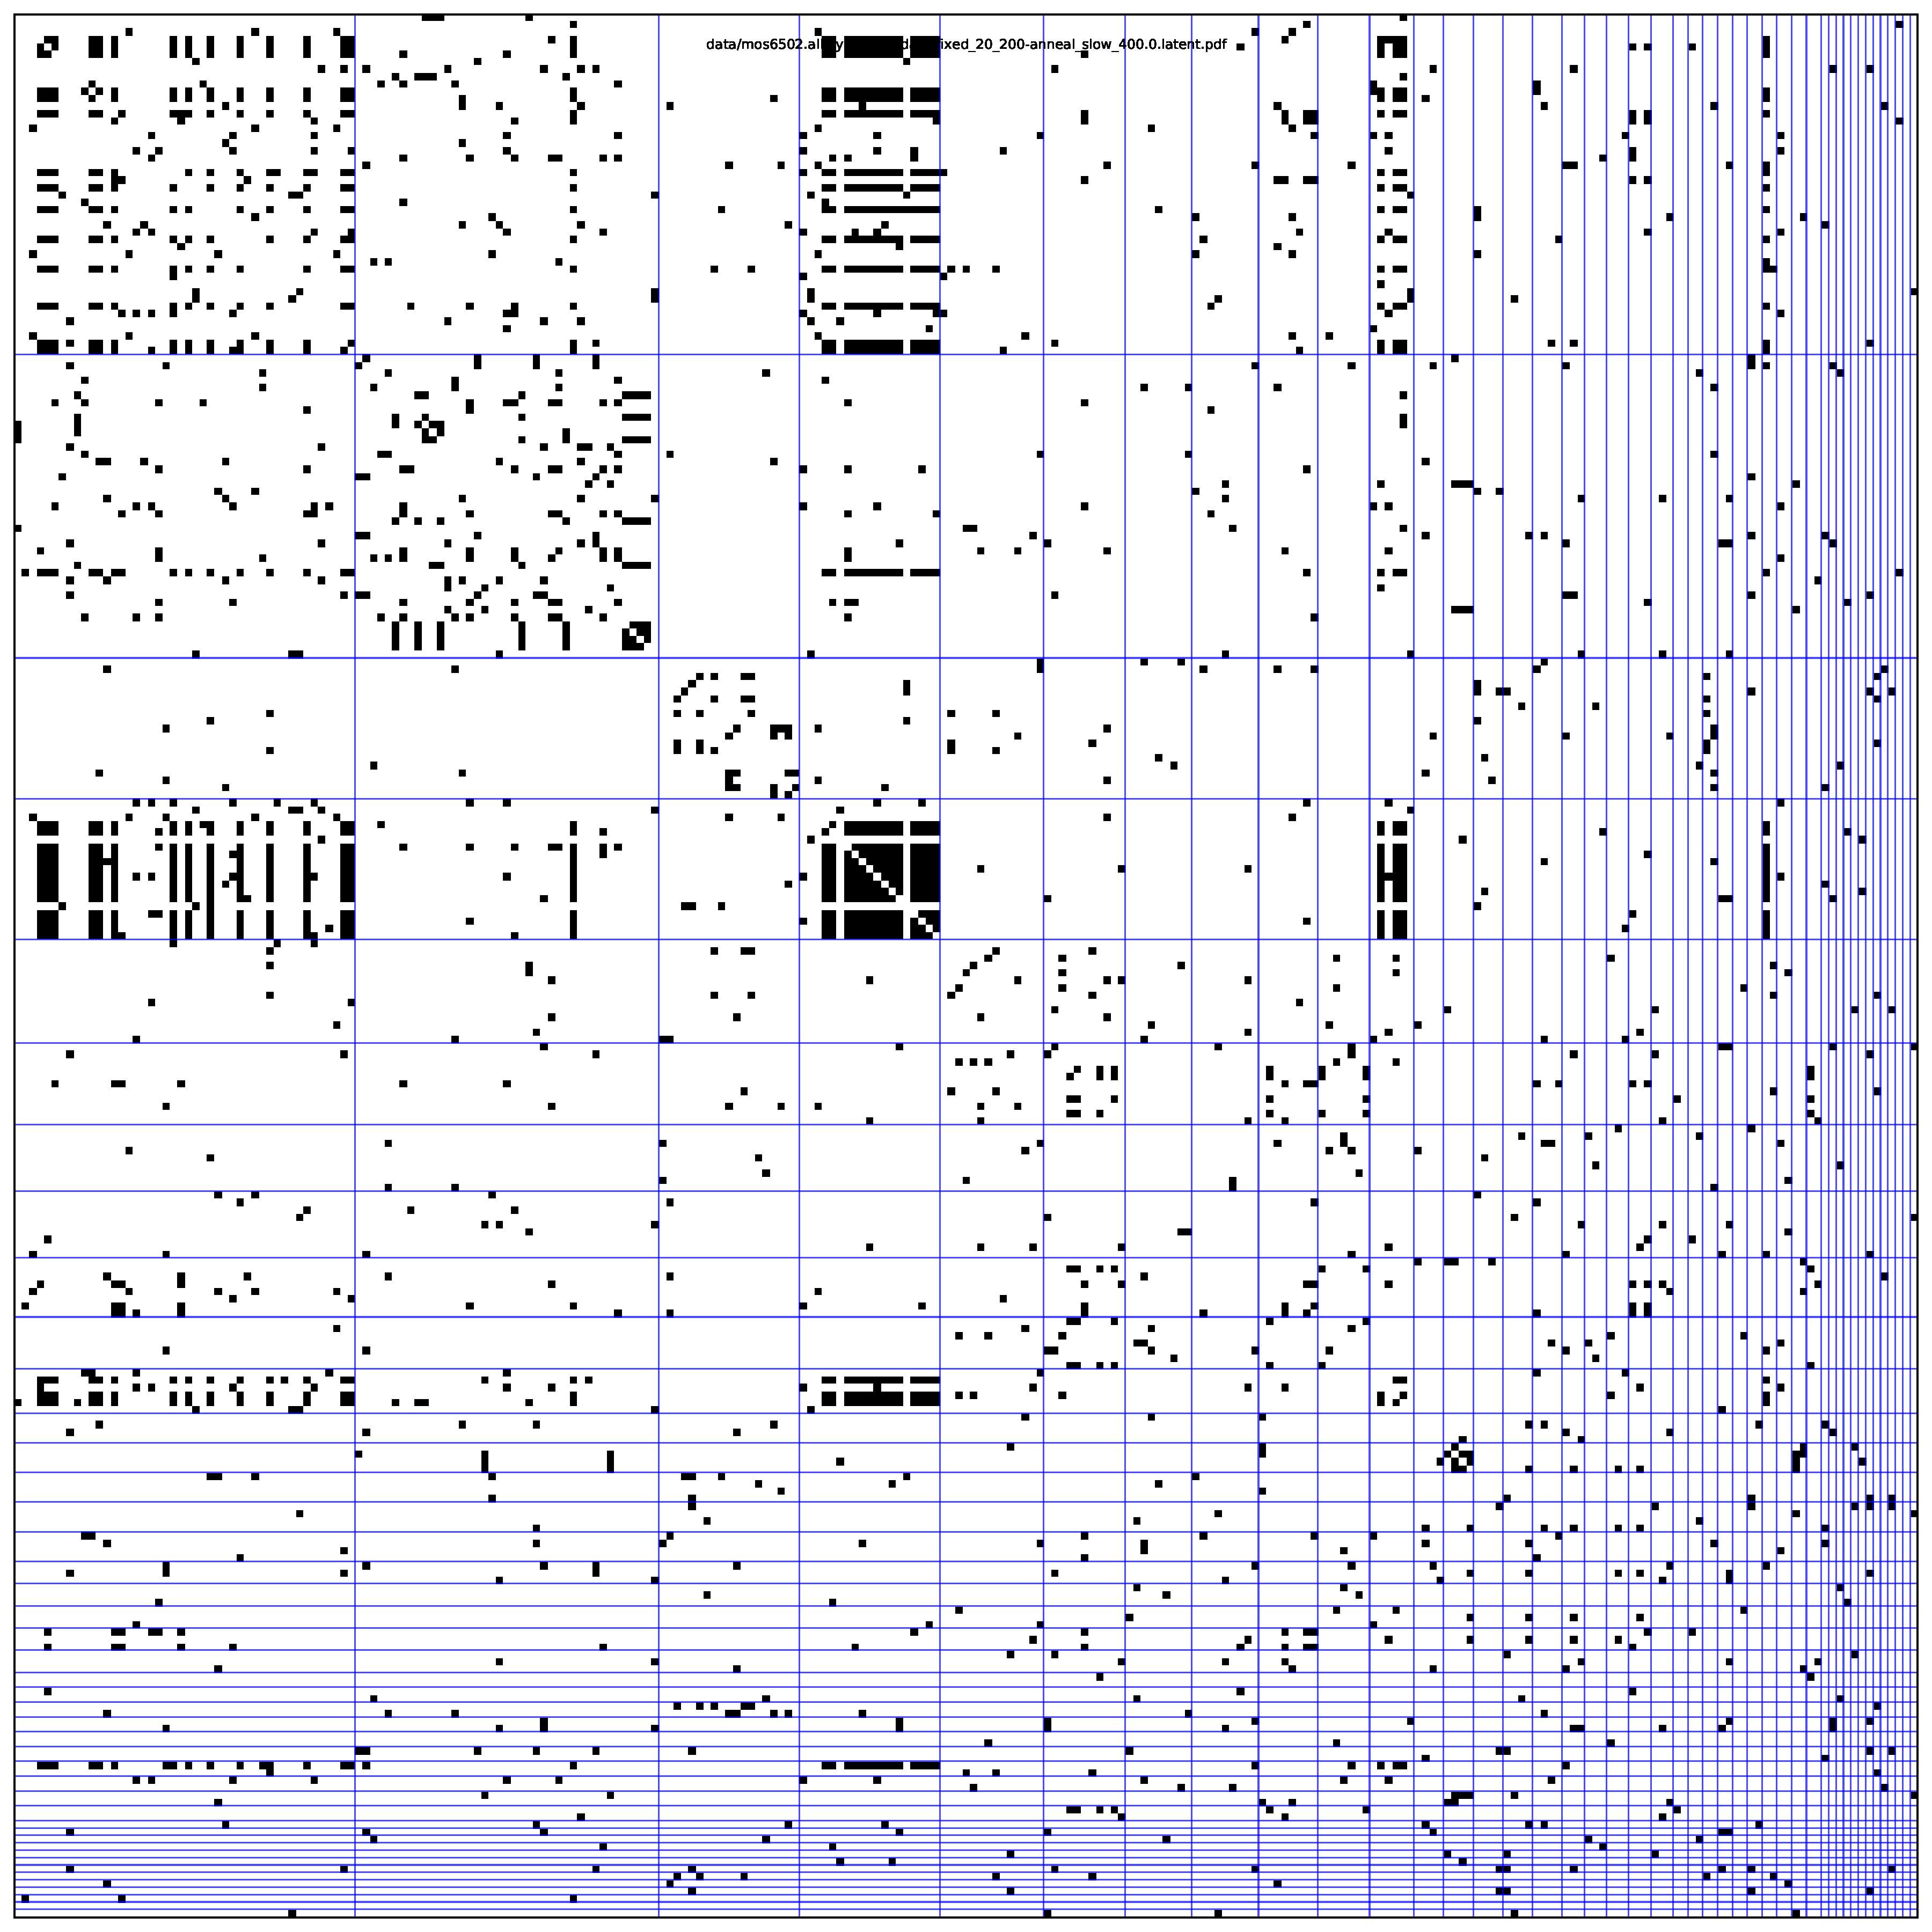
\includegraphics[width=\textwidth]{mos6502/mos6502.all.xysregs.ld.data-fixed_20_200-anneal_slow_400.0.latent.pdf}
  \caption{MOS 6502 XYS Register Latent}
\end{subfigure}
\caption{}
\label{}
\end{figure}

\todo[inline]{Show where those regions on the chip are}
\todo[inline]{Run on entire chip}
\todo[inline]{Other ways of encoding (multiple relations?) }
\todo[inline]{Run on entire chip with annealing}
\todo[inline]{interpret the damn latent structure}



\subsection{Job application data}

This data is from career builder. It contains who applied to what
jobs. This is our first non-graph example of a T1xT2 relation.


\section{Discussion}
Do we have enough data to make this work? 

Why does it fail sometimes? 

Tendency of stochastic block models to have block-diagonal structure -- that's not really how neuro works

Is type a static thing or a continuum? 


\section{Next Steps / Future Work}
How in gods name do we evaluate this? 

What abotu mixed membership models / better structural priors

What about incorporating additional metadata (``attribtue'' data)

Can we use something like a GP to learn the link function? 
Parametric link functions are nice, but you'd like to learn it from the data

How in gods name do we make this scale to 100k nodes? 
VB? spectral methods? Shitty heuristics? 

How in gods name do we make this hierarchical? 
We expect there to be hierarchy 

\printbibliography


\end{document}




